% Project report in the Vasavi College of Engineering format (Dept. of CSE), 2026.
% Body: Times New Roman 12 pt, 1.5 spacing; chapter headings 16 pt bold; section and subsection headings 12 pt bold;
% paragraph headings 14 pt bold; page numbers at bottom centre from the Introduction onwards; IEEE-style references.
% Typeset with Tectonic (XeTeX):  tools/tectonic/tectonic.exe main.tex   (run from report/project_report)
\documentclass[12pt,a4paper,oneside]{report}
\usepackage[left=3.5cm,right=2.5cm,top=2.5cm,bottom=2.5cm]{geometry}
\usepackage{fontspec}
\setmainfont{Times New Roman}
\setmonofont[Scale=0.86]{Courier New}
\usepackage{amsmath,amssymb}
\usepackage{booktabs,longtable,array,multirow,float,graphicx,xcolor,enumitem,setspace,titlesec,fancyhdr,caption,subcaption}
\usepackage{tikz}
\usetikzlibrary{arrows.meta,positioning,shapes.geometric,fit,calc}
\usepackage{algorithm}
\usepackage{algpseudocode}
\usepackage[hidelinks]{hyperref}
\usepackage{url}
\graphicspath{{./}{../}}
\newcommand{\NumNodes}{24,084,297}
\newcommand{\NumPairs}{72,394,470}
\newcommand{\NumAdj}{103,420,755}
\newcommand{\NumLabeled}{4,561}
\newcommand{\NumBad}{481}
\newcommand{\NumGood}{4,080}
\newcommand{\NumMiners}{3,953}
\newcommand{\NumFeat}{66}
\newcommand{\NumFeatEth}{32}
\newcommand{\NumFeatErc}{34}
\newcommand{\CovA}{74.5}
\newcommand{\CovB}{57.7}
\newcommand{\NoiseLo}{0.841}
\newcommand{\NoiseHi}{0.865}
\newcommand{\NoiseRange}{0.024}
\newcommand{\NoiseStd}{0.010}
\newcommand{\NoiseN}{4}
\newcommand{\BestWalks}{10}
\newcommand{\BestLen}{10}
\newcommand{\BestPRAUC}{0.947}
\newcommand{\TenTenPRAUC}{0.947}
\newcommand{\TenTenF}{0.893}
\newcommand{\TableTwoNtvPRAUC}{0.939}
\newcommand{\TFourPropPR}{0.837}
\newcommand{\TFourDynPR}{0.922}
\newcommand{\DynSeconds}{1598}
\newcommand{\PropSeconds}{454}
\newcommand{\DynAllPR}{0.930}
\newcommand{\TsneBadGoodKnn}{0.953}
\newcommand{\TsneBadGoodBal}{0.820}
\newcommand{\TsneBadGoodSil}{0.242}


% ------------------------------------------------------------------ project data (edit here only)
\newcommand{\ProjectTitle}{Reproducing and Extending RiskSEA: Scalable Graph Risk Scoring and Automated On-Chain Money Tracing for Fraud-Linked Exchange Identification}
\newcommand{\ProjectTitleShort}{Reproducing and Extending RiskSEA: Scalable Graph Risk Scoring and On-Chain Money Tracing}
\newcommand{\StudentA}{M. Krithika}\newcommand{\HtA}{1602-23-733-151}
\newcommand{\StudentB}{Satya Vaishnavi}\newcommand{\HtB}{1602-23-733-174}
\newcommand{\StudentC}{G. Vidya}\newcommand{\HtC}{1602-23-733-189}
\newcommand{\GuideName}{Mr. Kandi Trishaank}
\newcommand{\GuideDesignation}{Assistant Professor}
\newcommand{\HodName}{Dr. Nagaratna P. Hegde}
\newcommand{\Batch}{23}

% ------------------------------------------------------------------ formatting
\onehalfspacing
\setlength{\parindent}{1.0cm}
\setlength{\parskip}{0pt}
\setlist{itemsep=2pt,topsep=4pt,parsep=0pt}
\renewcommand{\arraystretch}{1.12}
\captionsetup{font={small,singlespacing},labelfont=bf,skip=6pt}
\setlength{\emergencystretch}{3em}
\titleformat{\chapter}[display]{\bfseries\fontsize{16}{20}\selectfont\centering}{\MakeUppercase{\chaptername}\ \thechapter}{8pt}{\MakeUppercase}
\titlespacing*{\chapter}{0pt}{-10pt}{22pt}
\titleformat{\section}{\bfseries\fontsize{12}{15}\selectfont}{\thesection}{0.7em}{}
\titleformat{\subsection}{\bfseries\fontsize{12}{15}\selectfont}{\thesubsection}{0.7em}{}
\titleformat{\subsubsection}{\bfseries\itshape\fontsize{12}{15}\selectfont}{\thesubsubsection}{0.7em}{}
\titleformat{\paragraph}[runin]{\bfseries\fontsize{14}{17}\selectfont}{}{0pt}{}[.\ ]
\titlespacing*{\section}{0pt}{14pt}{6pt}
\titlespacing*{\subsection}{0pt}{10pt}{4pt}
\titlespacing*{\paragraph}{0pt}{8pt}{0.4em}
\pagestyle{plain}
\renewcommand{\listtablename}{LIST OF TABLES}
\renewcommand{\listfigurename}{LIST OF FIGURES}
\renewcommand{\contentsname}{TABLE OF CONTENTS}
\setcounter{secnumdepth}{3}
\setcounter{tocdepth}{2}

% convenience macros
\newcommand{\vOK}{\textbf{reproduced}}
\newcommand{\vPart}{\textbf{partly}}
\newcommand{\vNo}{\textbf{not reproduced}}
\newcommand{\code}[1]{\texttt{#1}}
% a screenshot figure: \shot{file-stem}{caption}  (width = text width)
\newcommand{\shot}[2]{\begin{figure}[H]\centering\includegraphics[width=\textwidth]{shots/#1}\caption{#2}\label{fig:#1}\end{figure}}
\newcommand{\shotw}[3]{\begin{figure}[H]\centering\includegraphics[width=#3\textwidth]{shots/#1}\caption{#2}\label{fig:#1}\end{figure}}
% a generated table inside a float
\newcommand{\gentable}[3]{\begin{table}[H]\centering\small\singlespacing\setlength{\tabcolsep}{3pt}\input{#1}\caption{#2}\label{#3}\end{table}}

\begin{document}
% ============================================================== 1. COVER / TITLE PAGE
\begin{titlepage}
\thispagestyle{empty}
\begin{center}
\singlespacing
{\bfseries\fontsize{17}{22}\selectfont \MakeUppercase{\ProjectTitle}}\\[22pt]
{\bfseries\fontsize{16}{20}\selectfont A Project Report}\\[14pt]
{\fontsize{13}{17}\selectfont Submitted in partial fulfilment of the\\ Requirements for the award of the Degree of}\\[14pt]
{\bfseries\fontsize{16}{20}\selectfont BACHELOR OF ENGINEERING}\\[8pt]
{\bfseries\fontsize{13}{17}\selectfont IN}\\[8pt]
{\bfseries\fontsize{16}{20}\selectfont COMPUTER SCIENCE \& ENGINEERING}\\[14pt]
{\fontsize{13}{17}\selectfont By}\\[8pt]
{\bfseries\fontsize{14}{18}\selectfont \StudentA}\\{\fontsize{13}{17}\selectfont \HtA}\\[6pt]
{\bfseries\fontsize{14}{18}\selectfont \StudentB}\\{\fontsize{13}{17}\selectfont \HtB}\\[6pt]
{\bfseries\fontsize{14}{18}\selectfont \StudentC}\\{\fontsize{13}{17}\selectfont \HtC}\\[14pt]
{\fontsize{13}{17}\selectfont Under the guidance of}\\[8pt]
{\bfseries\fontsize{14}{18}\selectfont \GuideName}\\{\fontsize{13}{17}\selectfont \GuideDesignation}\\[14pt]

\includegraphics[width=2.6cm]{assets/logo.png}\\[10pt]
{\bfseries\fontsize{13}{17}\selectfont Department of Computer Science \& Engineering}\\
{\bfseries\fontsize{13}{17}\selectfont Vasavi College of Engineering (Autonomous)}\\
{\fontsize{12}{15}\selectfont (Affiliated to Osmania University)}\\
{\fontsize{12}{15}\selectfont Ibrahimbagh, Hyderabad-31}\\[8pt]
{\bfseries\fontsize{14}{18}\selectfont 2026}
\end{center}
\end{titlepage}

% ============================================================== 2. DECLARATION (department / guide copy)
\newcommand{\declhead}{%
\begin{center}\singlespacing
{\bfseries\fontsize{13}{17}\selectfont Vasavi College of Engineering (Autonomous)}\\
{\fontsize{12}{15}\selectfont (Affiliated to Osmania University)}\\
{\fontsize{12}{15}\selectfont Hyderabad-500 031}\\
{\bfseries\fontsize{13}{17}\selectfont Department of Computer Science \& Engineering}\\[10pt]

\includegraphics[width=2.3cm]{assets/logo.png}\\[16pt]
\end{center}}

\thispagestyle{empty}
\declhead
\begin{center}{\bfseries\fontsize{14}{18}\selectfont DECLARATION BY THE CANDIDATES}\end{center}
\vspace{8pt}
\noindent We, \StudentA, \StudentB{} and \StudentC, bearing hall ticket numbers \HtA, \HtB{} and \HtC{} respectively, hereby declare that the project report entitled ``\ProjectTitle'' under the guidance of \GuideName, \GuideDesignation, Department of Computer Science \& Engineering, VCE, Hyderabad, is submitted in partial fulfilment of the requirement for the award of the degree of Bachelor of Engineering in Computer Science \& Engineering.

\medskip
\noindent This is a record of bonafide work carried out by us and the results embodied in this project report have not been submitted to any other university or institute for the award of any other degree or diploma.

\vfill
\noindent{\small Note: (This is for Dept.\ / Guide copy only --- all the batch members)}
\begin{flushright}\singlespacing
\StudentA\\\HtA\\[8pt]
\StudentB\\\HtB\\[8pt]
\StudentC\\\HtC
\end{flushright}
\clearpage

% ============================================================== 3. DECLARATION (personal copies, one per student)
\newcommand{\personaldecl}[2]{%
\thispagestyle{empty}
\declhead
\begin{center}{\bfseries\fontsize{14}{18}\selectfont DECLARATION BY THE CANDIDATE}\end{center}
\vspace{8pt}
\noindent I, #1, bearing hall ticket number #2, hereby declare that the project report entitled ``\ProjectTitle'' under the guidance of \GuideName, \GuideDesignation, Department of Computer Science \& Engineering, VCE, Hyderabad, is submitted in partial fulfilment of the requirement for the award of the degree of Bachelor of Engineering in Computer Science \& Engineering.

\medskip
\noindent This is a record of bonafide work carried out by me and the results embodied in this project report have not been submitted to any other university or institute for the award of any other degree or diploma.

\vfill
\begin{flushright}\singlespacing
#1\\#2
\end{flushright}
\clearpage}
\personaldecl{\StudentA}{\HtA}
\personaldecl{\StudentB}{\HtB}
\personaldecl{\StudentC}{\HtC}

% ============================================================== 4. BONAFIDE CERTIFICATE
\thispagestyle{empty}
\declhead
\begin{center}{\bfseries\fontsize{14}{18}\selectfont BONAFIDE CERTIFICATE}\end{center}
\vspace{8pt}
\noindent This is to certify that the project entitled ``\ProjectTitle'' being submitted by \StudentA, \StudentB{} and \StudentC, bearing \HtA, \HtB{} and \HtC{} respectively, in partial fulfilment of the requirements for the award of the degree of Bachelor of Engineering in Computer Science \& Engineering is a record of bonafide work carried out by them under my guidance.

\vspace{110pt}
\noindent\begin{tabular}{@{}p{7.2cm}p{7cm}@{}}
\GuideName & \HodName\\
\GuideDesignation & Professor \& HEAD\\
Internal Guide & Dept.\ of CSE
\end{tabular}
\clearpage

% ============================================================== 5. ACKNOWLEDGEMENT  (roman numbering starts here)
\pagenumbering{roman}
\setcounter{page}{1}
\begin{center}{\bfseries\fontsize{16}{20}\selectfont ACKNOWLEDGEMENT}\end{center}
\vspace{6pt}
\noindent We express our sincere gratitude to our internal guide, \GuideName, \GuideDesignation, Department of Computer Science \& Engineering, for the guidance, patience and encouragement that shaped this project from the first reading of the baseline paper to the final demonstration. The direction to reproduce a published system before improving it, and to state plainly where our results differ from the paper, came from this guidance.

We thank \HodName, Professor and Head of the Department of Computer Science \& Engineering, for providing the environment and the freedom to take on a problem of this scale, and the Principal of Vasavi College of Engineering (Autonomous) for the institutional support extended to the project batch.

We are grateful to the faculty of the department for the courses that made this work possible, in particular those on data structures, algorithms, machine learning, databases and software engineering, and to our project review committee for their suggestions during the interim reviews.

This work builds on the efforts of others whom we acknowledge here: the authors of RiskSEA, whose paper we reproduced; the authors of the textbook on blockchain transaction data analytics whose tracing, attribution and risk-pattern chapters shaped the extension; the maintainers of the open-source libraries we relied on; and the organisations that publish open data, namely the Google BigQuery public Ethereum dataset, the community-maintained Ethereum label lists and the public OFAC sanctions list.

Finally we thank our parents and friends for their support and understanding during the long working sessions this project demanded.

\vspace{26pt}
\begin{flushright}\singlespacing
\StudentA\\\HtA\\[8pt]
\StudentB\\\HtB\\[8pt]
\StudentC\\\HtC
\end{flushright}
\clearpage

% ============================================================== 6. ABSTRACT
\begin{center}{\bfseries\fontsize{16}{20}\selectfont ABSTRACT}\end{center}
\vspace{6pt}
\noindent Victims of cryptocurrency fraud report a wallet address, but the money has usually moved through several anonymous addresses before it reaches an exchange, the only place that holds customer records and can freeze an account. Following that trail by hand takes investigators days. This project has two parts. First, we independently reproduce RiskSEA (Agarwal et al., Coinbase), a scalable graph-embedding risk score for Ethereum addresses, using only the paper's text and public data: Ethereum blocks up to 5\,000\,000, a graph of \NumNodes{} addresses and \NumLabeled{} labeled addresses, on a single laptop. The hyperparameter findings reproduce, dynamic node2vec beats embedding propagation in all three checkpoints with a clear margin at the last, and the paper's headline claim that graph embeddings add substantially to behavioural features does not reproduce on our data, for reasons we trace to our easier, miner-dominated labels.

Second, because RiskSEA scores wallets but does not follow money, we design and build CryptoTrace, a working prototype that starts from a victim-reported wallet and finds the first service that received the funds. It replaces a trained global embedding with a local, directed, time-respecting, value-weighted propagation (TTR-lite); stops at labeled exchanges, mixers, decentralized-exchange contracts and busy hubs; infers exchange deposit addresses with a sweep rule; tags laundering patterns with explainable rules; and returns evidence as paths of real transactions. It is delivered as a FastAPI service with live event streaming and a React application that animates the search. On two documented hacks the tracer reaches the published destinations (99.8\% of the KuCoin funds at the Tornado Cash 100 ETH pool; 99.98\% of the Cryptopia funds at the EtherDelta contract), and on a real phishing-labeled wallet it attributes 90.9\% of the funds to 29 deposit addresses that sweep into one exchange, where a blind two-hop search finds nothing. Each case costs under \$0.15 of BigQuery scanning, and later runs are free through a cache. The report also documents the limits: ETH external transfers only, three cases rather than a full benchmark, inferred rather than confirmed exchange links, and the pending work needed to turn the prototype into a service.

\medskip
\noindent\textbf{Keywords:} blockchain analytics, Ethereum, money tracing, node2vec, RiskSEA, exchange attribution, taint analysis, fraud investigation.
\clearpage

% ============================================================== 7--9. CONTENTS, TABLES, FIGURES
\singlespacing
\tableofcontents
\clearpage
\listoftables
\clearpage
\listoffigures
\clearpage
\onehalfspacing


% ================================================================== body: page numbers start here
\clearpage
\pagenumbering{arabic}
\setcounter{page}{1}
\chapter{Introduction}
\label{ch:intro}

\section{Overview}
Public blockchains such as Ethereum record every transfer of value permanently and openly, yet an address carries no name. This is both their strength and their weakness. A fraudster who receives stolen funds is not identified by the ledger, and the ledger makes it easy to split, forward and recombine those funds across many addresses within minutes. At the same time, every one of those movements is visible to anyone who can read the chain, so the trail exists; the difficulty is following it quickly and presenting it in a form that an investigator, an exchange compliance officer or a court can check.

This project starts from a published system for the first half of that problem and extends it towards the second half. The published system is \emph{RiskSEA} (Agarwal et al., Coinbase) \cite{risksea}, which gives every Ethereum address a risk score between 0 and 1 by combining behavioural statistics of its transfers with a graph embedding produced by node2vec \cite{node2vec}. Its distinctive contribution is scale: it keeps an embedding for hundreds of millions of addresses up to date as the chain grows. We first reproduce that system end to end on a single laptop and compare every table and figure of the paper with what we obtain (Chapters~\ref{ch:analysis}, \ref{ch:impl} and~\ref{ch:results}). We then observe that RiskSEA, however well reproduced, does not answer the question an investigator asks after a victim reports a wallet: \emph{where did the money go, and which exchange can freeze it?} To answer that question we design and build \emph{CryptoTrace}, a working prototype that follows funds forward from a reported wallet, stops at the first service that received them, and returns the evidence as a path of real transactions.

\section{Motivation}
Cyber-fraud complaints that involve cryptocurrency share a pattern. The victim sends funds to an address supplied by the scammer. Within minutes or hours the funds are forwarded to a second address, split into equal parts, forwarded again and finally deposited at a cryptocurrency exchange, where they are converted or withdrawn. Three facts make the exchange the pivotal point.
\begin{enumerate}
\item An exchange holds identity (KYC) records for its customers, so a deposit address at an exchange can be tied to a person.
\item An exchange can freeze an account if it receives a timely, well-evidenced request.
\item Public label lists name an exchange's main wallets, but they almost never name the thousands of per-customer \emph{deposit addresses}. These have to be inferred from behaviour.
\end{enumerate}
Today the tracing is done by an analyst who opens a block explorer, reads the outgoing transfers of the reported wallet, picks the ones that look relevant and repeats for each recipient. A hop takes minutes; a realistic case takes days; and the result is a set of screenshots, not a reproducible analysis. Commercial tracing tools exist, but they are closed, expensive and give no way to see why a path was chosen. A method that is fast, explainable and open is therefore valuable, and the research literature, summarised in Chapter~\ref{ch:analysis}, shows that local, directed, time-aware tracing is the right family of methods for it, while whole-graph embedding methods are slow and weak at tracing.

\section{Problem Definition}
\label{sec:problem}
The problem statement that frames this work is:

\begin{quote}\itshape
Real-time identification of fraud-linked cryptocurrency exchanges from victim-reported suspect wallet addresses through automated blockchain analytics: ingest reported wallets, trace the funds across hops, identify the nearest exchange or virtual-asset service provider (VASP) that received them, detect laundering patterns and intermediary (mule) wallets, categorise wallet risk, support more than one chain, and deliver the result through dashboards and an API that can be integrated with law-enforcement reporting platforms.
\end{quote}

Stated as a computational problem: given a source address $s$, an incident time window $[t_0,t_1)$ and the public transaction history of a chain, output (i)~the set of terminal entities $T$ where the funds from $s$ ended up within the window, (ii)~for each $t\in T$ the estimated share of the funds that reached it, its type (exchange, exchange deposit address, mixer, decentralized exchange, unlabeled service) and a confidence, and (iii)~for each $t$ a time-ordered path of real transactions from $s$ to $t$, so that every claim can be verified independently.

\section{Objectives}
The work was carried out against two sets of objectives that follow each other.

\paragraph{Part A: reproduce the baseline.}
\begin{enumerate}
\item Implement every component the RiskSEA paper describes, from its text alone.
\item Re-run its experiments (Tables~II--IV and Figures~5--13) as faithfully as public data and one laptop allow.
\item State clearly where we had to deviate and quantify the effect of each deviation.
\item Leave a trusted, tested baseline that later improvements can be measured against.
\end{enumerate}

\paragraph{Part B: extend it to the investigator's question.}
\begin{enumerate}
\item Build a tracer that starts from a reported wallet and follows funds forward in time, by amount.
\item Identify the first labeled exchange, or infer an exchange deposit address, reached by the funds; and stop honestly at mixers, decentralized-exchange contracts and busy hubs.
\item Return evidence as paths of real transactions plus explainable laundering-pattern tags.
\item Validate the tracer on documented incidents and compare it with simpler strategies on the same data.
\item Keep the cost of data access low and bounded, and make re-runs free.
\item Deliver it as an API and an interactive application suitable for a live demonstration, with every limit stated in the interface.
\end{enumerate}

\section{Scope}
\subsection{In scope}
\begin{itemize}
\item The Ethereum chain: external ETH transfers read from the public BigQuery dataset.
\item Reproduction of RiskSEA on Ethereum blocks 0--5\,000\,000 (to early 2018) with public labels.
\item Forward tracing from a single reported wallet within a window of up to 120 days.
\item Attribution to labeled exchanges, mixers, a decentralized-exchange contract, sanctioned addresses, inferred exchange deposit addresses and unlabeled hubs.
\item Three tracing strategies (ours, classic taint tracking and blind breadth-first search) on three cases: two documented hacks and one real phishing-labeled wallet.
\item A FastAPI backend, a React interface and a printable investigator report.
\end{itemize}
\subsection{Out of scope (listed as pending work in Chapter~\ref{ch:pending})}
\begin{itemize}
\item Internal contract transfers, ERC-20 tokens and stablecoins, and other chains such as Bitcoin, Tron or BNB Chain; cross-chain bridges.
\item Real-time ingestion: the public dataset lags the chain, so the prototype is near-real-time at best.
\item Integration with the SAHYOG and NCRP platforms: no specification was available, so these are recorded as requirements to clarify, not built.
\item A full multi-case benchmark such as the 20-case evaluation reported in the literature; our three cases are a smoke test.
\end{itemize}

\section{Summary of the Work Done}
Table~\ref{tab:workdone} lists, in the order they happened, what was done in this project. Each item is described in the chapter noted in the last column.

\begin{table}[H]
\centering\small\singlespacing
\begin{tabular}{r p{8.4cm} p{3.4cm}}
\toprule
\textbf{\#} & \textbf{Work item} & \textbf{Chapter}\\
\midrule
1 & Review of the RiskSEA paper; assessment of how far it can be implemented and what would be needed & \ref{ch:analysis}\\
2 & End-to-end implementation plan and workflow; decision log started (24 entries) & \ref{ch:analysis}, \ref{ch:impl}\\
3 & BigQuery dry runs, billing caps, authentication, parallel resumable download & \ref{ch:impl}\\
4 & Label sourcing and audit (Etherscan-derived lists, OFAC, miners) & \ref{ch:analysis}\\
5 & Graph build (DuckDB, top-200), core selection, behavioural features (66 columns) & \ref{ch:impl}\\
6 & node2vec at laptop scale, embedding propagation, dynamic node2vec, partitioned walk generator & \ref{ch:impl}\\
7 & Experiments: Table~II, hyperparameter sweep (Table~III), Table~IV, t-SNE figures, noise measurement & \ref{ch:results}\\
8 & Four silent-corruption bugs found and fixed; 61 automated tests & \ref{ch:impl}\\
9 & Comparative study of paper versus reproduction (data constraints, scorecard, gaps) & \ref{ch:results}\\
10 & Study of the tracing literature; decision to use RiskSEA as a baseline, not as the whole system; research gaps & \ref{ch:analysis}\\
11 & CryptoTrace design: architecture, data model, engines, attribution, API, interface & \ref{ch:design}\\
12 & CryptoTrace implementation and 17 further automated tests (78 in total) & \ref{ch:impl}\\
13 & Validation on the KuCoin and Cryptopia incidents; discovery and trace of a real phishing-labeled wallet & \ref{ch:results}\\
14 & Interface polish: grouped findings, demo guide, shortcuts, responsive layout & \ref{ch:results}\\
15 & Complete screenshot set of every screen, and this report & \ref{ch:results}, Appendix\\
\bottomrule
\end{tabular}
\caption{Work done, in order.}
\label{tab:workdone}
\end{table}

\section{Organization of the Report}
Chapter~\ref{ch:analysis} analyses the existing methods, summarises the literature, sets the data and resource constraints of the reproduction against the paper's, states the research gaps and gives an overview of the proposed system with its requirements. Chapter~\ref{ch:design} gives the design: the reproduction pipeline, the CryptoTrace architecture, the data model, the data layer, the tracing and attribution engines, the API and the interface. Chapter~\ref{ch:impl} gives the algorithms in pseudo-code and the implementation details, the bugs found and the testing. Chapter~\ref{ch:results} presents all results: the reproduction against the paper, the tracing results for each case, the comparison of strategies, the cost, and a walk through every screen of the application. Chapter~\ref{ch:pending} lists the pending work. The references follow, and the appendices hold the decision log, the full list of addresses found, reproduction commands and the full-page screenshots.

\chapter{System Analysis and Overview of the Proposed System}
\label{ch:analysis}

\section{Existing System}
\subsection{Manual investigation with block explorers}
An investigator who receives a victim-reported address opens a public block explorer, reads the list of transactions, selects the outgoing transfers that look relevant and repeats the process for every recipient. The investigator has to decide at every hop whether a recipient is a pass-through account, an exchange deposit address, a mixer or an ordinary user, usually from memory and from scattered public tags. The effort grows with the number of hops and with the fan-out of the funds. The output is a set of screenshots and notes that another analyst cannot easily reproduce.

\subsection{Rule-based and commercial tracing tools}
Commercial blockchain-analytics suites automate part of this work and maintain large proprietary label databases. Their label coverage is their main advantage. Their drawbacks for this problem are cost, closed algorithms that offer no explanation of why a path was followed, and, for many users, no way to run the analysis on their own data. We did not have access to any of them, and we do not compare against them.

\subsection{Machine-learning wallet scoring}
The research and industry systems closest to this work score wallets. RiskSEA \cite{risksea}, the paper we reproduced, is the clearest example: it outputs a risk score for each address from behavioural features and a graph embedding. Scoring answers ``how risky is this address'', which is useful for compliance screening. It does not follow money, it does not respect the direction or the timing of transfers (node2vec walks are undirected and untimed), and it does not name the exchange that received the funds. The textbook that guided the extension \cite{textbook} reports that embedding-based methods applied to tracing needed more than 24 hours per case or missed targets, which is the practical reason not to use them for the tracing step.

\section{Literature Survey}
\label{sec:litsurvey}
Table~\ref{tab:lit} summarises the families of methods that bear on the problem and how each was used in this project. Citations to the textbook refer to its chapters on entity identification, risk patterns, heterophily in transaction graphs, streaming graph embedding and transaction tracing.

\begin{table}[H]
\centering\small\singlespacing
\begin{tabular}{p{2.9cm} p{4.7cm} p{4.7cm}}
\toprule
\textbf{Method} & \textbf{Idea and strength} & \textbf{Weakness for tracing; use here}\\
\midrule
node2vec \cite{node2vec} & Biased second-order random walks, then skip-gram, give each node a vector that reflects its neighbourhood. Good for classification. & Undirected, untimed, assumes similar nodes are adjacent. Reproduced as the RiskSEA baseline; not used for tracing.\\
dynnode2vec \cite{dynnode2vec} & Incremental node2vec: walk only from changed nodes and continue training from previous weights. & Same assumptions as node2vec. Reproduced as ``dynamic node2vec'' (Chapter~\ref{ch:results}).\\
RiskSEA \cite{risksea} & Random forest over behavioural features and node2vec, with embedding propagation and incremental updates to reach every address. & A wallet score, not a tracer. Reproduced; planned as the risk-model module.\\
Taint analysis (haircut, poison) \cite{textbook} & Spread taint forward from the source in proportion to value (haircut) or to every output (poison). Simple and explainable. & No ranking, so the output grows quickly; ignores timing. Implemented as the Haircut baseline.\\
Blind BFS \cite{textbook} & Follow every neighbour to a fixed depth. & Output explodes; a depth cap of two means it stops before funds reach an exchange. Implemented as a baseline.\\
Personalised PageRank (APPR) \cite{pagerank,appr} & Local push algorithm that ranks nodes by relevance to a source and touches only a small part of the graph. & Undirected relevance, no time. Its push mechanism is the basis of our engine.\\
TRacer / TTR \cite{tracer,textbook} & Adapts the push idea to transactions: a tendency to follow outflows, weighting by amount, temporal reasoning (funds follow only later transfers) and token redirection through swaps. & Designed for exactly this problem. Implemented in reduced form as TTR-lite.\\
Label propagation, Louvain \cite{textbook} & Community methods that spread labels over the whole graph. & Cost grows with the graph; poor recall at tracing in the published comparison.\\
Heterophily-aware models \cite{textbook} & Observe that on transaction graphs adjacent nodes often have different labels (edge homophily about 0.28 reported), so smoothing-based models underperform. & Motivates abandoning embedding smoothing for the tracing step; a path for the future risk model.\\
\bottomrule
\end{tabular}
\caption{Methods considered and how each is used in this project.}
\label{tab:lit}
\end{table}

\subsection{Published comparison of tracing methods}
The textbook \cite{textbook} compares the methods above on 20 real incidents across three chains. We reproduce its table in Table~\ref{tab:bookbench} because it is the evidence behind our choice of method; these are published numbers, not ours.

\begin{table}[H]
\centering\small\singlespacing
\begin{tabular}{p{5.0cm} r r r r}
\toprule
\textbf{Method} & \textbf{Recall (\%)} & \textbf{Accounts (K)} & \textbf{Depth} & \textbf{Time (h)}\\
\midrule
TRacer (ranked local search) & 92.31 & 0.87 & 5.05 & 0.65\\
APPR (personalised PageRank) & 71.92 & 0.66 & 3.60 & 0.51\\
BFS (depth 2) & 77.02 & 52.50 & 2.00 & 0.05\\
Poison taint (depth 2) & 70.06 & 41.45 & 2.00 & 0.03\\
Haircut taint & 58.85 & 10.35 & 4.15 & 0.01\\
Label propagation (LPA) & 67.76 & 682.30 & 10.35 & 1.76\\
Louvain communities & 51.27 & 111.84 & 9.75 & 1.69\\
Ethprivacy (features) & 0.01 & 1.89 & 1.10 & 1.78\\
Metapath2Vec / Ethprivacy (embeddings) & --- & --- & --- & $>24$\\
\bottomrule
\end{tabular}
\caption{Published comparison on 20 real cases (source: the textbook, transaction-tracing chapter). Recall is the share of target accounts found; accounts is the number of accounts in the output, in thousands; time is the runtime in hours. A ranked local search reaches the highest recall while reviewing about 870 accounts; blind BFS reviews about 52\,500 for lower recall.}
\label{tab:bookbench}
\end{table}

\section{The Baseline Paper in Brief}
\label{sec:paper}
\textbf{Task.} Given an Ethereum address, output a risk score in $[0,1]$. Ground truth has two classes: \emph{Risk-1} (addresses involved in illegal activity such as phishing, scams or theft) and \emph{Risk-0} (exchanges, miners, government). If sources disagree the higher risk wins.

\textbf{Model.} A random-forest classifier over three feature sets: behavioural features of ETH transactions, behavioural features of ERC-20 transfers (amounts, timestamps, frequencies), and a node2vec embedding of the transaction graph. The intuition is that malicious addresses spread funds through tightly knit clusters of helper addresses, which an embedding of graph neighbourhoods can capture.

\textbf{Scaling problems and the two proposed solutions.} node2vec is transductive (no embedding for unseen addresses), expensive at 266\,M nodes, and must be recomputed as the chain grows. The paper offers:
\begin{enumerate}
\item \emph{Embedding propagation:} train node2vec on a core set of 30\,M addresses and give every other address the aggregate of up to five randomly sampled one-hop core neighbours (78\% of addresses reached).
\item \emph{DynN2VChain:} an incremental version of node2vec (after dynnode2vec \cite{dynnode2vec}): walks are generated only from addresses that changed, over the whole current graph, and the skip-gram model is trained further from its previous weights. Random walks are generated by a horizontally scalable split--apply--combine procedure over a neighbour list capped at the top 200 neighbours.
\end{enumerate}

\textbf{Reported results.} Table~II: behavioural features, propagated node2vec and both (F$_1$ 0.718, 0.738, 0.851). Table~III and Figures~5--9: a hyperparameter sweep (best: $p=q=1$, 10 walks of length 10). Table~IV and Figure~10: dynamic node2vec outperforms propagation at every checkpoint. Figures~11--13: t-SNE plots in which labels form clusters.

\section{Data and Resource Constraints: Paper versus Reproduction}
\label{sec:constraints}
Before any result is compared, this section lays out how our inputs differ from the paper's. The differences are large, and they shape how every later number should be read.

\subsection{Side-by-side comparison}
{\small\singlespacing
\begin{longtable}{p{2.7cm} p{5.4cm} p{6.0cm}}
\caption{Data, scale and resource differences between the paper and this reproduction.}\label{tab:constraints}\\
\toprule
\textbf{Aspect} & \textbf{Paper} & \textbf{This reproduction}\\
\midrule\endfirsthead
\toprule
\textbf{Aspect} & \textbf{Paper} & \textbf{This reproduction}\\
\midrule\endhead
\bottomrule\endfoot
Chain period & Ethereum up to Sept.\ 2023; checkpoints at 5\,M, 8\,M, 10\,M and 16\,M blocks & Blocks 0--5\,000\,000 (to early 2018)\\
Graph size & $\approx$266\,M addresses (275\,M in the conclusion) & \NumNodes{} addresses; \NumPairs{} directed address pairs; \NumAdj{} adjacency entries after the top-200 cap\\
Transfers used & ETH transactions and ERC-20 transfers & Same: 148.7\,M ETH transactions (no internal traces) aggregated to 56.4\,M pairs; 20.3\,M ERC-20 address--token pairs\\
Label count & 129\,012 (43\,334 Coinbase-internal + 85\,678 external) & 10\,044 public labels, of which \NumLabeled{} appear in the graph: \NumBad{} bad and \NumGood{} good\\
Label sources & Coinbase internal data; external sources not disclosed & Public only: Etherscan-derived \code{eth-labels}, OFAC list, block miners\\
Good class & Exchanges, miners, government & \NumMiners{} miners (97\%) and 127 exchanges\\
Bad class & Illegal activity (phishing, scam, theft, \dots) & 474 Etherscan phishing/hack addresses and 7 OFAC-sanctioned\\
Class balance & ``Balanced representation'' sought; counts not given & 10.5\% bad ($481/4\,561$)\\
Compute & Databricks CPU clusters (i3.8xlarge, r5.16xlarge, r5.xlarge); a V100 GPU for the 30\,M-address model & One laptop: 16 cores, 15.7\,GiB RAM, no GPU\\
Embedding memory & 30\,M addresses held in GPU memory & 2.5\,M-node core in RAM (a dense 24\,M $\times$ 128 float32 matrix alone would take 12\,GB)\\
Core set & 30\,M of 266\,M (11.3\%) & 2.5\,M of 24.1\,M (10.4\%)\\
Distributed walks & MapReduce on a cluster & Partitioned neighbour store with a process pool; output verified bit-identical to the in-memory generator; not run on a cluster\\
Incremental updates & Daily, 5\,M $\to$ 16\,M blocks & Every 250\,K blocks, 4.0\,M $\to$ 5.0\,M, on a 3\,M-node universe\\
Sweep graph & 30\,M-address subsample & The 2.5\,M-node core subgraph\\
Edge weights & Interaction counts used to rank top-$K$ neighbours & Counts in the global graph; time-sliced snapshots are unweighted\\
Unspecified details & Embedding dimension, skip-gram settings, forest settings, split, threshold, behavioural feature list & Chosen by us (Appendix~\ref{app:decisions})\\
Metrics & P/R/F$_1$ (Table~II); ``AUC'' (Tables~III--IV), not defined & P/R/F$_1$ at 0.5, PR-AUC (area under the precision--recall curve), ROC-AUC\\
Uncertainty & None reported & 95\% confidence intervals over 5 splits; retraining noise measured\\
\end{longtable}}

\subsection{Labels in detail}
Ground-truth labels are the single biggest difference. Table~\ref{tab:labels} shows what we could assemble from public sources and how much of it is usable.
\begin{table}[H]
\centering\small\singlespacing
\begin{tabular}{l c r r}
\toprule
Source & class & labeled & present in graph (blocks $\leq$ 5M)\\
\midrule
Etherscan phishing/hack (eth-labels) & bad & 5,590 & 474\\
OFAC sanctioned addresses & bad & 123 & 7\\
Block miners (from \texttt{blocks.miner}) & good & 3,959 & 3,953\\
Etherscan exchanges (eth-labels) & good & 372 & 127\\
\midrule
Total usable after merge & & & 481 bad / 4,080 good\\
\bottomrule
\end{tabular}
\caption{Public label sources and how many labeled addresses exist in our graph.}
\label{tab:labels}
\end{table}
Three features of this label set matter for interpreting results.
\begin{enumerate}
\item \textbf{Timing.} Of 5\,590 Etherscan phishing/hack addresses only 474 are active by block 5\,000\,000; most appear later. Bad addresses are scarce early: only 1 is present at block 2.0\,M, 36 at 4.0\,M, 262 at 4.5\,M and 481 at 5.0\,M. This forced us to evaluate time-resolved experiments only from 4.0\,M onward.
\item \textbf{Composition of the good class.} Miners dominate (97\%). Miners have an unusual structure (regular payouts to many recipients), so ``bad versus good'' is plausibly easier here than in the paper's setting, which also includes exchanges and government addresses.
\item \textbf{Provenance.} The phishing/hack and exchange labels derive from Etherscan tags via a public repository whose scraping may conflict with Etherscan's terms of use. We asked for and received approval before downloading, used them for research only, kept the raw files out of version control, and flag this as a caveat on redistribution.
\end{enumerate}

\subsection{What these constraints imply}
\begin{itemize}
\item \textbf{Absolute scores are not comparable.} Our behavioural baseline scores F$_1$ 0.956 against the paper's 0.718; we attribute much of this to the easy, miner-heavy negative class rather than to better features.
\item \textbf{Small bad class.} A 20\% test split contains about 96 bad addresses, so single-split metrics are noisy; we report confidence intervals and warn where a row rests on very few positives.
\item \textbf{Smaller, older graph.} Our graph ends in early 2018, five years before the paper's, when Ethereum had far fewer contracts and none of the later DeFi patterns, and it is about 11 times smaller. Propagation coverage and the value of graph structure may differ.
\item \textbf{One machine.} Memory forced a subsampled core and a 3\,M-node universe; wall-clock times are not comparable with a cluster.
\end{itemize}

\section{Research Gaps}
\label{sec:gaps}
Reading the baseline against the tracing literature gives five gaps, each of which a design decision of CryptoTrace answers. Table~\ref{tab:gaps} pairs them.

\begin{table}[H]
\centering\small\singlespacing
\begin{tabular}{r p{6.0cm} p{6.0cm}}
\toprule
\textbf{\#} & \textbf{Gap} & \textbf{Our response}\\
\midrule
1 & Embeddings are slow and weak at tracing: global methods took over 24 hours per case or missed targets, while a targeted local search found 92\% of targets in 0.65 hours reviewing about 870 accounts. & Local ranked propagation from the reported wallet (TTR-lite); no training.\\
2 & Heterophily: scam wallets transact with exchanges and ordinary victims, yet node2vec assumes similar nodes are adjacent and walks on the undirected graph. & Directed, time-respecting, value-weighted flow instead of embedding smoothing.\\
3 & Single chain, batch data, pre-2018 history: real cases need recent data, live feeds and cross-chain bridges. & A provider interface (Edge model) that another chain can implement; live BigQuery mode with caps; cross-chain listed as pending.\\
4 & Missing deposit-address labels: public lists tag exchange hot wallets, not customer deposit addresses. & Sweep rule that infers deposit addresses from behaviour, marked as inferred.\\
5 & Auditable evidence: investigators need transaction hashes, amounts and timestamps, not a black-box score. & Evidence path of real transactions for every finding, with confidence and stated limits.\\
\bottomrule
\end{tabular}
\caption{Research gaps and the corresponding design response.}
\label{tab:gaps}
\end{table}

\paragraph{Why RiskSEA alone is not enough.} RiskSEA is a strong baseline for wallet risk scoring, for exchange classification (our reproduction separates miners from exchanges with silhouette 0.457) and for data infrastructure (BigQuery extraction, top-$K$ graph build, incremental updates, label audit and a leakage-aware test harness). It is not the baseline for the whole system, because the core task is directed path tracing and entity attribution, which RiskSEA does not perform. We therefore keep it as the planned risk-model module and build the tracer separately.

\section{Proposed System}
CryptoTrace is a pipeline of small modules with one job each: intake of a reported wallet and window; a chain adapter that turns the chain into a stream of timed, valued transfers; an edge cache; a label store; a tracing engine; an attribution engine; a typology engine; a case file and report; a dashboard and API; and a benchmark harness (Chapter~\ref{ch:design}). The key properties are:
\begin{itemize}
\item \textbf{Starts from the complaint.} A single reported wallet and a time window, not a pre-scored graph.
\item \textbf{Local and incremental.} Only the neighbourhoods the search touches are fetched, one query per hop.
\item \textbf{Direction, time and amount.} Funds follow transfers that happen after they arrive, split in proportion to value.
\item \textbf{Attributes, then stops.} It stops at labeled exchanges, mixers, DEX contracts and busy hubs, and infers deposit addresses.
\item \textbf{Explains itself.} Evidence paths with transaction hashes, rule-based pattern tags, confidence levels and a visible list of limits.
\item \textbf{Cheap.} The first fetch of a case costs cents; re-runs cost nothing.
\end{itemize}

\section{Requirements}
\subsection{Functional requirements}
\begin{enumerate}[label=FR\arabic*.]
\item Accept a source address, an incident window and a tracing strategy, validate them, and run the trace as a background job.
\item Fetch the neighbourhood of an address from the chain provider, capped to the largest transfers per direction and a minimum value.
\item Cache every fetched neighbourhood so repeated runs, parameter changes and replays need no new queries.
\item Expand the frontier round by round, following only time-consistent transfers, and report the share of funds explained after each round.
\item Stop at labeled exchanges, mixers, sanctioned addresses and DEX contracts, infer exchange deposit addresses, and flag unlabeled high-activity hubs.
\item Return, for each destination, the share and estimated amount of funds, its type, a confidence level and a path of real transactions.
\item Tag laundering patterns: pass-through accounts, fan-out, fan-in, peeling chains and fast hops.
\item Stream events to the interface while the trace runs.
\item Compare strategies on a case on equal terms (destinations reached, accounts to audit, transfers considered, depth, rounds, run time, cost).
\item Produce a printable investigator report including the list of addresses to ask an exchange to freeze.
\end{enumerate}
\subsection{Non-functional requirements}
\begin{enumerate}[label=NFR\arabic*.]
\item \textbf{Cost control:} a dry run before spending, a per-query byte cap and a per-trace budget (30\,GiB); no credentials stored in the repository.
\item \textbf{Honesty:} every inferred result is labeled as inferred; every limit of the data is visible in the interface and in the report.
\item \textbf{Determinism and testability:} engines depend only on a provider interface, so they can be tested without network access.
\item \textbf{Responsiveness:} cached cases replay in seconds; the interface works at projector resolutions (1280$\times$720 and up).
\item \textbf{Portability:} the same engine code must work for another chain by supplying another provider.
\end{enumerate}

\subsection{Hardware and software requirements}
\begin{table}[H]
\centering\small\singlespacing
\begin{tabular}{p{3.4cm} p{9.6cm}}
\toprule
\textbf{Item} & \textbf{Specification used}\\
\midrule
Machine & Windows 11 laptop, 16 cores, 15.7\,GiB RAM, no GPU\\
Language and runtime & Python 3.12 (analysis and backend), Node.js 24 (frontend build)\\
Data and analytics & Google BigQuery public \code{crypto\_ethereum} dataset; DuckDB; NumPy, pandas, PyArrow\\
Machine learning & scikit-learn (random forest, t-SNE, metrics), gensim (skip-gram), Numba (walk generation)\\
Backend & FastAPI, Uvicorn, Pydantic, server-sent events; SQLite for the edge cache\\
Frontend & React with Vite, framer-motion, d3-force, Recharts, lucide-react; an HTML canvas for the animated graph\\
Testing & pytest (78 tests)\\
Typesetting & Tectonic (XeTeX) for this report and the comparative study\\
\bottomrule
\end{tabular}
\caption{Hardware and software environment.}
\label{tab:env}
\end{table}

\section{Feasibility and Cost}
\paragraph{Technical.} All components are open-source or free-tier, and the work fits on one laptop. The reproduction needed a subsampled core and a 3\,M-node universe because of memory; the tracer needs no training and runs in under a second on cached data.

\paragraph{Economic.} BigQuery bills by bytes scanned (on-demand pricing is per TiB; the first TiB each month is free). We assumed a list price of \$6.25 per TiB, which should be checked against current pricing. The reproduction extraction scanned 48.6\,GiB, which matched its dry run. The tracing prototype scanned 9.51\,GiB for the Cryptopia case, 3.87\,GiB for KuCoin and 19.9\,GiB for the phishing case, about \$0.06, \$0.02 and \$0.12. Finding the phishing example required one exploration query of 29.9\,GiB (about \$0.18), and the total BigQuery spend across the whole MVP was roughly \$0.6. Every cached re-run costs nothing.

\paragraph{Operational.} Public BigQuery data lags the chain, so the prototype is near-real-time at best. A live deployment needs a node, an RPC provider or a commercial feed; that is part of the pending work.

\paragraph{Legal and ethical.} The addresses analysed are public on-chain data. The Etherscan-derived labels come from a scraped public repository, flagged in the decision log; any redistribution requires checking those terms. Every result is presented as an investigative lead, not as proof of identity.

\chapter{System Design}
\label{ch:design}

\section{Design of the Reproduction Pipeline}
The reproduction is a file-based pipeline in which every stage reads and writes files, so any stage can be re-run alone (Figure~\ref{fig:pipeline}). BigQuery extraction aggregates the public Ethereum tables on the server so that only compact tables are downloaded. A DuckDB build turns those tables into a top-200 neighbour graph. A core-set selection and node2vec training stage produces embeddings, which propagation or the dynamic variant extend to all addresses. A random forest combines embeddings with behavioural features and public labels, and an evaluation stage regenerates the paper's tables and figures.

\begin{figure}[H]
\centering
\resizebox{\textwidth}{!}{%
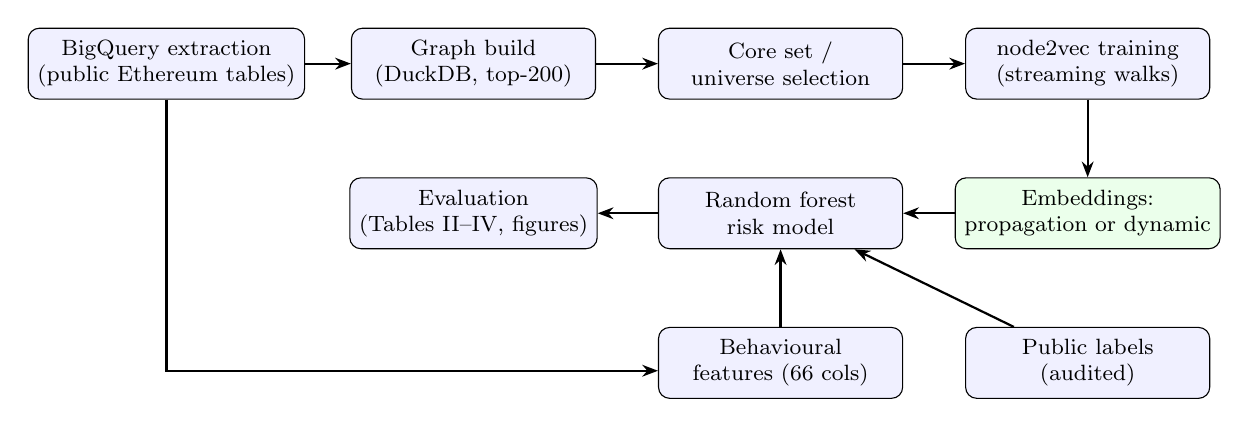
\begin{tikzpicture}[box/.style={draw,rounded corners,align=center,minimum height=9mm,minimum width=3.1cm,font=\footnotesize,fill=blue!6},
  arr/.style={-{Stealth[length=2mm]},thick}]
\node[box] (bq) at (0,0) {BigQuery extraction\\(public Ethereum tables)};
\node[box] (gr) at (3.9,0) {Graph build\\(DuckDB, top-200)};
\node[box] (co) at (7.8,0) {Core set /\\universe selection};
\node[box] (tr) at (11.7,0) {node2vec training\\(streaming walks)};
\node[box,fill=green!8] (em) at (11.7,-1.9) {Embeddings:\\propagation or dynamic};
\node[box] (rf) at (7.8,-1.9) {Random forest\\risk model};
\node[box] (ev) at (3.9,-1.9) {Evaluation\\(Tables II--IV, figures)};
\node[box] (fe) at (7.8,-3.8) {Behavioural\\features (66 cols)};
\node[box] (lb) at (11.7,-3.8) {Public labels\\(audited)};
\draw[arr] (bq)--(gr); \draw[arr] (gr)--(co); \draw[arr] (co)--(tr); \draw[arr] (tr)--(em);
\draw[arr] (em)--(rf); \draw[arr] (rf)--(ev); \draw[arr] (fe)--(rf); \draw[arr] (lb)--(rf);
\draw[arr] (bq) |- ([yshift=-1mm]fe.west);
\end{tikzpicture}}
\caption{Overview of the reproduction pipeline. Every stage reads and writes files.}
\label{fig:pipeline}
\end{figure}

\section{Architecture of CryptoTrace}
CryptoTrace is organised as a pipeline of modules with plain data interfaces: a complaint enters on the left, and a case file and dashboard leave on the right. A label store feeds the attribution step, and a benchmark harness sits beside the pipeline. Figure~\ref{fig:arch} shows the modules; solid boxes are built and exercised, dashed boxes are designed but pending. The same structure is drawn by the application's System page from a data file (\code{architecture.py}), so the interface can never show a module that does not exist.

\begin{figure}[H]
\centering
\resizebox{\textwidth}{!}{%
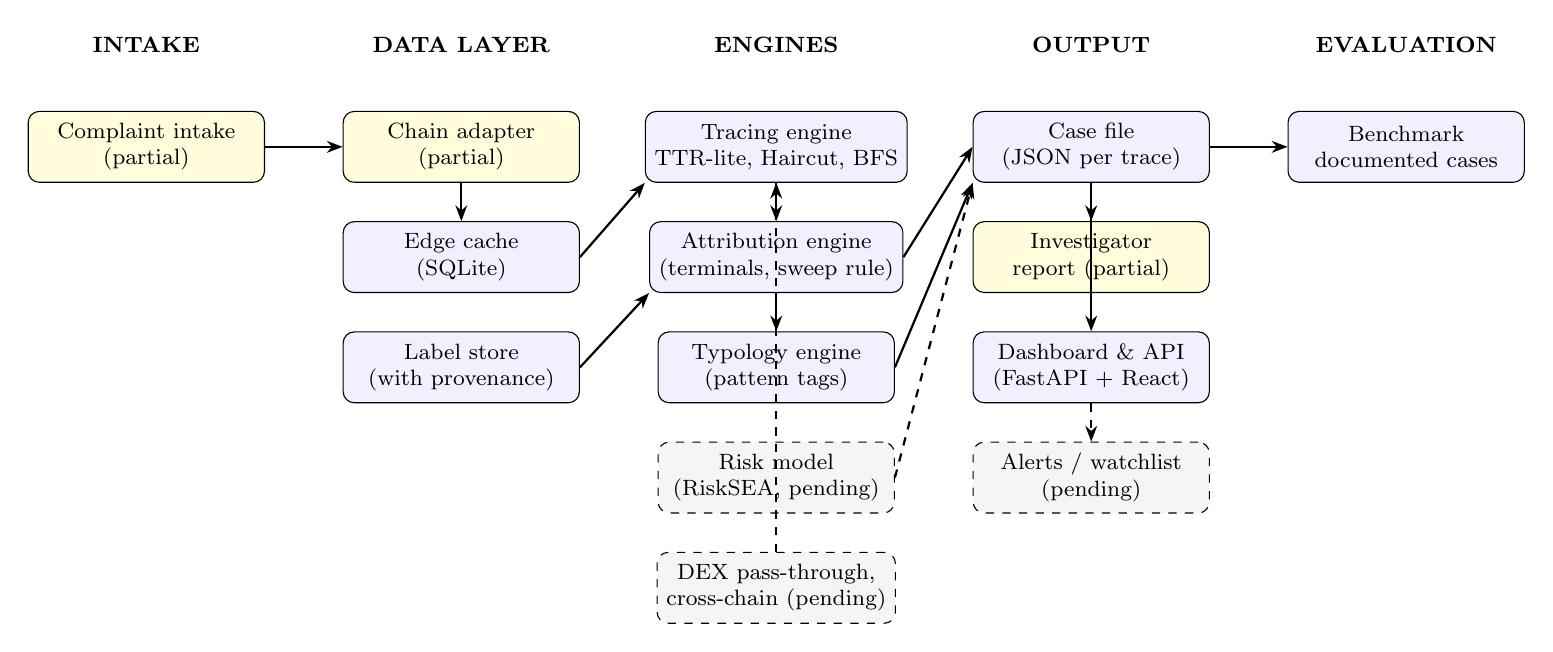
\begin{tikzpicture}[
  m/.style={draw,rounded corners,align=center,minimum height=9mm,minimum width=3.0cm,font=\footnotesize,fill=blue!6},
  p/.style={draw,dashed,rounded corners,align=center,minimum height=9mm,minimum width=3.0cm,font=\footnotesize,fill=gray!8},
  pa/.style={draw,rounded corners,align=center,minimum height=9mm,minimum width=3.0cm,font=\footnotesize,fill=yellow!14},
  hd/.style={font=\footnotesize\bfseries},
  arr/.style={-{Stealth[length=2mm]},thick}]
\node[hd] at (0,3.7) {INTAKE}; \node[hd] at (4,3.7) {DATA LAYER}; \node[hd] at (8,3.7) {ENGINES}; \node[hd] at (12,3.7) {OUTPUT}; \node[hd] at (16,3.7) {EVALUATION};
\node[pa] (intake) at (0,2.4) {Complaint intake\\(partial)};
\node[pa] (adapter) at (4,2.4) {Chain adapter\\(partial)};
\node[m]  (cache)   at (4,1.0) {Edge cache\\(SQLite)};
\node[m]  (labels)  at (4,-0.4) {Label store\\(with provenance)};
\node[m]  (tracing) at (8,2.4) {Tracing engine\\TTR-lite, Haircut, BFS};
\node[m]  (attr)    at (8,1.0) {Attribution engine\\(terminals, sweep rule)};
\node[m]  (typ)     at (8,-0.4) {Typology engine\\(pattern tags)};
\node[p]  (risk)    at (8,-1.8) {Risk model\\(RiskSEA, pending)};
\node[p]  (dex)     at (8,-3.2) {DEX pass-through,\\cross-chain (pending)};
\node[m]  (case)    at (12,2.4) {Case file\\(JSON per trace)};
\node[pa] (report)  at (12,1.0) {Investigator\\report (partial)};
\node[m]  (dash)    at (12,-0.4) {Dashboard \& API\\(FastAPI + React)};
\node[p]  (alerts)  at (12,-1.8) {Alerts / watchlist\\(pending)};
\node[m]  (bench)   at (16,2.4) {Benchmark\\documented cases};
\draw[arr] (intake)--(adapter); \draw[arr] (adapter)--(cache); \draw[arr] (cache.east)--(tracing.south west);
\draw[arr] (labels.east)--(attr.south west); \draw[arr] (tracing)--(attr); \draw[arr] (attr)--(typ);
\draw[arr] (typ.east)--(case.south west); \draw[arr] (attr.east)--(case.west); \draw[arr] (case)--(report); \draw[arr] (case.south)--(dash.north);
\draw[arr] (case.east)--(bench.west);
\draw[arr,dashed] (risk.east)--(case.south west); \draw[arr,dashed] (dex.north)--(tracing.south);
\draw[arr,dashed] (dash)--(alerts);
\end{tikzpicture}}
\caption{CryptoTrace architecture. Solid: built and exercised by the benchmark cases; yellow: partly built; dashed: designed but pending.}
\label{fig:arch}
\end{figure}

\begin{table}[H]
\centering\small\singlespacing
\begin{tabular}{p{3.2cm} p{2.1cm} p{7.6cm}}
\toprule
\textbf{Module} & \textbf{Status} & \textbf{Role and limit}\\
\midrule
Complaint intake & partial & Takes a wallet, window and strategy through the API; batch import and SAHYOG/NCRP integration are pending.\\
Chain adapter & partial & Ethereum external ETH transfers via BigQuery; internal transfers, ERC-20 and other chains pending.\\
Edge cache & live & SQLite store of every fetched neighbourhood; re-runs cost nothing.\\
Label store & live & 372 exchange, 5\,594 known-bad, 123 sanctioned, 4 mixer pools and 1 DEX (curated) addresses, each with provenance.\\
Tracing engine & live & TTR-lite plus the Haircut and BFS baselines.\\
Attribution engine & live & Labeled stops, deposit-sweep rule, unlabeled hub guard.\\
Typology engine & live & Zero-out, fan-out, fan-in, peel and fast-hop tags.\\
Risk model & planned & RiskSEA reproduction exists offline; not wired in.\\
DEX pass-through & planned & Needs the BigQuery traces table (internal transfers).\\
Cross-chain & planned & Needs bridge-event matching.\\
Case file & live & One JSON per trace with nodes, edges, destinations, paths, tags, warnings, events.\\
Investigator report & partial & Printable view live; standard-format export pending.\\
Dashboard \& API & live & FastAPI with live event streaming; React application.\\
Alerts / watchlist & planned & Needs a live feed.\\
Benchmark & live & Compares strategies on documented cases.\\
\bottomrule
\end{tabular}
\caption{The fifteen modules of CryptoTrace and their status.}
\label{tab:modules}
\end{table}

\section{Data Model}
Everything the engines do is expressed in terms of one structure, the \emph{Edge}: a single on-chain transfer, directed, timed and valued. A different chain only needs a different provider that yields Edges.

\begin{table}[H]
\centering\small\singlespacing
\begin{tabular}{p{2.6cm} p{4.0cm} p{6.4cm}}
\toprule
\textbf{Structure} & \textbf{Fields} & \textbf{Meaning}\\
\midrule
Edge & src, dst, eth, ts, blk, tx & One transfer: sender, receiver, value in ETH, Unix time, block number, transaction hash.\\
Label & kind, name, source & What an address is (exchange, mixer, sanctioned, bad, dex) and where that knowledge came from.\\
FetchResult & edges, degree, queries, bytes\_billed, cache\_hits & What one provider call returns: transfers, the true in/out degree before the per-node cap, and cost counters.\\
TraceParams & alpha, beta, epsilon, max\_rounds, min\_eth, hub\_degree, time\_respecting, top\_k, bfs\_depth, max\_frontier & The algorithm's parameters (defaults 0.15, 0.8, $10^{-3}$, 8, 0.01 ETH, 3000, true, 200, 2, 300).\\
TraceEvent & round, kind, nodes, edges, info & One animation frame: start, expand, absorb or done, with the round's frontier, residual and cost counters.\\
\bottomrule
\end{tabular}
\caption{Core data structures.}
\label{tab:datamodel}
\end{table}

The result of a trace (the \emph{case file}) contains: the nodes with their role (source, intermediate, terminal, upstream), label, depth, rank, share and pattern tags; the edges with role (forward or backward) and share; the terminals with type, share, estimated ETH, depth, first-arrival time, confidence and evidence path; the statistics (rounds, queries, bytes billed, cache hits, seconds); the warnings; and the full event log used by the interface to replay the search.

\section{Data Layer Design}
\subsection{One query per hop}
Tracing asks for the neighbourhood of a few addresses at a time. Each search round is therefore one BigQuery query against the public \code{transactions} table, returning at most the 200 largest transfers per address and direction. This keeps the cost independent of how large the chain is. The query (Listing~\ref{lst:hopsql}) filters by a time window so BigQuery can prune partitions, drops dust below \code{min\_eth}, and uses a window function to keep the top-$k$ per node and direction while also returning the true degree, which the attribution engine uses to recognise busy hubs.

\begin{figure}[H]
\centering\footnotesize
\begin{minipage}{0.97\textwidth}
\begin{verbatim}
WITH e AS (          -- transfers touching the requested nodes
  SELECT hash AS tx, from_address AS src, to_address AS dst,
         CAST(value AS FLOAT64)/1e18 AS eth,
         UNIX_SECONDS(block_timestamp) AS ts, block_number AS blk
  FROM `bigquery-public-data.crypto_ethereum.transactions`
  WHERE block_timestamp >= TIMESTAMP_SECONDS(@t0)   -- prunes partitions
    AND block_timestamp <  TIMESTAMP_SECONDS(@t1)
    AND to_address IS NOT NULL AND value > 0
    AND (from_address IN UNNEST(@nodes)
         OR to_address IN UNNEST(@nodes))
), ends AS (         -- one row per (node, direction)
  SELECT src AS node,'out' AS dir,tx,src,dst,eth,ts,blk
    FROM e WHERE src IN UNNEST(@nodes)
  UNION ALL
  SELECT dst AS node,'in' AS dir,tx,src,dst,eth,ts,blk
    FROM e WHERE dst IN UNNEST(@nodes)
)
SELECT node,dir,tx,src,dst,eth,ts,blk,
       COUNT(*) OVER (PARTITION BY node,dir) AS deg  -- true degree
FROM ends WHERE eth >= @min_eth
QUALIFY ROW_NUMBER() OVER (PARTITION BY node,dir
                           ORDER BY eth DESC) <= @k   -- top-k
\end{verbatim}
\end{minipage}
\caption{The per-hop query (abridged from the implementation).}
\label{lst:hopsql}
\end{figure}

\subsection{Cache, cost control and the provider interface}
The provider is the only component that talks to BigQuery. It stores every fetched neighbourhood in a SQLite database keyed by the minimum value, the per-node cap and the end of the window; an address is therefore fetched at most once per configuration, and a later request for an earlier start time triggers a re-fetch of only that address. Four controls bound the spend: (i)~a dry run reports the bytes a query would scan before anything is billed; (ii)~every job carries a \code{maximum\_bytes\_billed} cap of 40\,GiB; (iii)~the provider refuses to start a query that would take the total for one trace over a 30\,GiB budget; and (iv)~in \emph{cache-only} mode a request for an address that was never fetched raises a clear error instead of silently spending. The engines always request edges from the start of the incident window and decide themselves which are time-consistent, so the provider never filters by time and the time-respecting switch is real. A second provider holds a fixed edge list in memory for tests and replays.

\subsection{Label store}
The label store maps an address to a \emph{kind} and a \emph{name} and records the source of every label. It is loaded from public files: Etherscan-derived exchange and phishing/hack lists, the OFAC sanctions list, and a small curated list. The curated list holds the four Tornado Cash pool addresses (each verified on-chain to receive a single fixed denomination of 0.1, 1, 10 or 100 ETH), the EtherDelta contract (curated from public knowledge and marked \emph{unverified on-chain}) and the Yobit.net wallet printed in the textbook's case study. Figure~\ref{fig:label_store} shows the counts.

\begin{figure}[H]
\centering
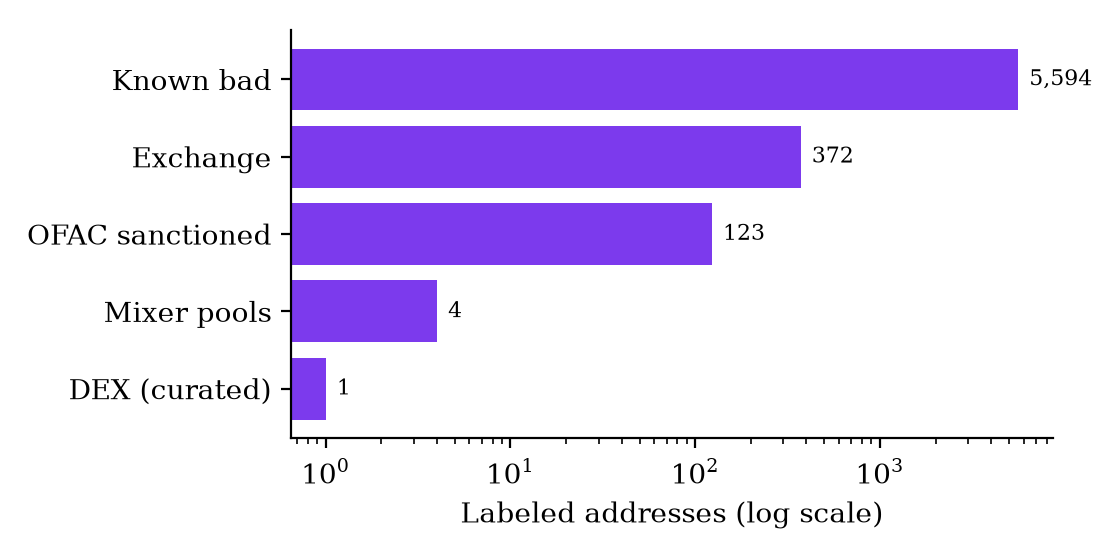
\includegraphics[width=0.78\textwidth]{figs/label_store.png}
\caption{Labeled addresses by kind in the label store (log scale).}
\label{fig:label_store}
\end{figure}

\section{Tracing Engine Design}
\subsection{Idea}
The tracer treats the reported wallet as holding 100\% of an unexplained quantity, the \emph{residual}, and repeatedly pushes residual along transfers to the next accounts, in proportion to value, until the residual left unexplained is negligible or the funds reach a service. Two quantities travel together. The \emph{rank} measures relevance to the source, decays with distance and decides which accounts are expanded next. The \emph{share} estimates the fraction of the source's funds that reached an account and is what the report states.

\subsection{TTR-lite formulation}
Let $r(v)$ be the residual at account $v$, initialised to $r(s)=1$ at the source $s$, and let $\alpha,\beta,\epsilon$ be the parameters of Table~\ref{tab:datamodel}. In each round every account with $r(v)>\epsilon$ that is not a terminal or an upstream account is expanded, highest residual first, at most 300 per round. For an expanded account $v$ that first received funds at time $a(v)$:
\begin{align}
F(v)&=\{(v\to u,x,t):t\ge a(v)\}, & B(v)&=\{(w\to v,x,t):t<a(v)\},\\
\mathrm{rank}(v) &\mathrel{+}= \alpha\, r(v),\\
r(u) &\mathrel{+}= (1-\alpha)\,\beta\, r(v)\,\frac{x}{\sum_{F(v)}x} && \forall\,(v\to u,x,t)\in F(v),\\
r(w) &\mathrel{+}= (1-\alpha)(1-\beta)\, r(v)\,\frac{x}{\sum_{B(v)}x} && \forall\,(w\to v,x,t)\in B(v).
\end{align}
The four ideas taken from the literature are visible here. \emph{Tracing tendency}: $\beta$ of the residual goes forward along outflows and $1-\beta$ backward along inflows. \emph{Weighted pollution}: the split is proportional to the amount transferred. \emph{Temporal reasoning}: forward transfers must occur at or after the funds arrived, and backward transfers strictly before, so the transfer on which the funds arrived is never walked backwards. \emph{Token redirection} through swaps is not implemented in the prototype because it handles ETH only. In parallel, a pending share $\sigma(v)$ is split by the same forward fractions, $\sigma(u)\mathrel{+}=\sigma(v)\,x/\sum_{F(v)}x$, and is the quantity reported as ``share of funds''. If an account has no forward or no backward transfers, all of its residual goes the other way.

\subsection{Baselines}
\textbf{Haircut taint} carries a sender's tainted share forward in proportion to value and stops when the remaining taint is below a threshold; it is forward-only, has no ranking and no backward pass. \textbf{Blind BFS} follows every outflow of every discovered account to a fixed depth (two, as in the literature), ignoring time and amount; shares are split uniformly and exist only so the comparison table can be filled. Both baselines use the same provider, terminals and result builder as TTR-lite, so differences in the comparison come from the search strategy alone.

\section{Attribution Design}
\subsection{Terminals}
A \emph{terminal} is an account where tracing stops because the funds reached a service. Labeled exchanges, mixers, sanctioned addresses and DEX contracts stop the trace immediately, without fetching their (huge) neighbourhood. Two further terminals are inferred.

\paragraph{Exchange deposit address (sweep rule).} Public lists tag an exchange's hot wallets but rarely its customer deposit addresses, which an exchange creates by the thousand and \emph{sweeps} into its hot wallet. An unlabeled account $v$ is classified as a deposit address of exchange $X$ if, among its outflows within 48 hours of the funds arriving, at least 80\% of the value goes to labeled wallets of $X$ and the outflows go to at most three recipients. The result carries \emph{medium} confidence and the label ``inferred''. Figure~\ref{fig:sweep} shows the pattern.

\begin{figure}[H]
\centering
\resizebox{0.9\textwidth}{!}{%
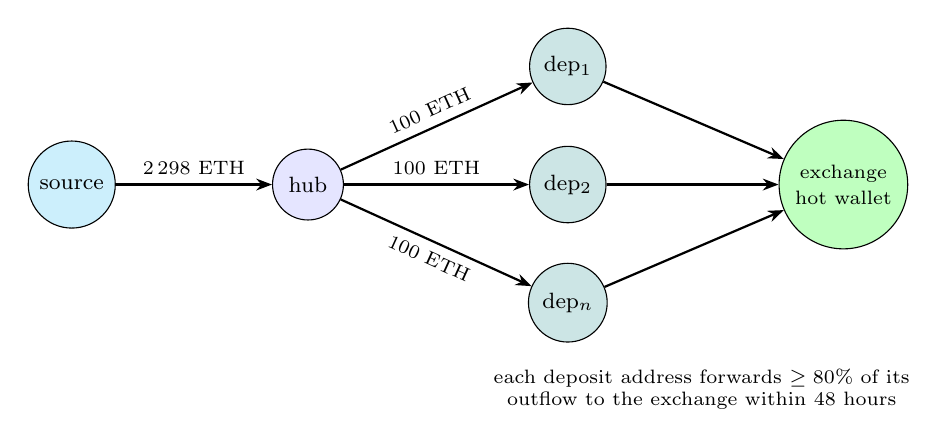
\begin{tikzpicture}[n/.style={draw,circle,minimum size=9mm,font=\footnotesize,align=center},
  arr/.style={-{Stealth[length=2mm]},thick}, lab/.style={font=\scriptsize,midway,above}]
\node[n,fill=cyan!20] (s) at (0,0) {source};
\node[n,fill=blue!10] (a) at (3,0) {hub};
\node[n,fill=teal!20] (d1) at (6.3,1.5) {dep$_1$};
\node[n,fill=teal!20] (d2) at (6.3,0) {dep$_2$};
\node[n,fill=teal!20] (d3) at (6.3,-1.5) {dep$_n$};
\node[n,fill=green!25,minimum size=13mm] (x) at (9.8,0) {\scriptsize exchange\\\scriptsize hot wallet};
\draw[arr] (s)--(a) node[lab] {2\,298 ETH};
\draw[arr] (a)--(d1) node[lab,sloped] {100 ETH};
\draw[arr] (a)--(d2) node[lab] {100 ETH};
\draw[arr] (a)--(d3) node[lab,sloped,below] {100 ETH};
\draw[arr] (d1)--(x); \draw[arr] (d2)--(x); \draw[arr] (d3)--(x);
\node[font=\scriptsize,align=center] at (8.0,-2.6) {each deposit address forwards $\ge 80\%$ of its\\outflow to the exchange within 48 hours};
\end{tikzpicture}}
\caption{The deposit sweep pattern that the attribution engine looks for.}
\label{fig:sweep}
\end{figure}

\paragraph{Unlabeled service hub.} An unlabeled account with more than 3\,000 transfers in the window is treated as a service (a pool, a payment processor or an exchange wallet that no list names). The trace stops there with \emph{low} confidence and the account is flagged for manual review, because following funds through such an account is guesswork.

\subsection{Confidence}
Labeled exchanges, mixers and sanctioned addresses carry high confidence, since the label itself is public knowledge. A DEX contract and an inferred exchange deposit address carry medium confidence (the label is curated, or the link is inferred). An unlabeled hub carries low confidence.

\subsection{Evidence paths}
For each terminal the engine reports the time-ordered chain of real transactions from the source that carries the largest share. Starting from the source, it scans all forward edges in time order and keeps, for each account, the best score so far, where the score of an edge is the score of its sender times the fraction of the sender's outflow that the edge carries; an edge is usable only if it occurs after the funds reached its sender. Walking the predecessor links back from the terminal gives the path. This is a dynamic program over the time-sorted edge list.

\section{Typology Design}
The typology engine tags accounts of the traced subgraph with simple rules that need no training data and can be read by an investigator.
\begin{itemize}
\item \textbf{Zero-out:} forwards at least 90\% of what it received within 24 hours (a pass-through bridge account).
\item \textbf{Fan-out:} sends to five or more different recipients within 24 hours (splitting or layering).
\item \textbf{Fan-in:} receives from five or more different senders (aggregation).
\item \textbf{Peel:} passes at least 70\% of the funds in one transfer and keeps or spreads a small remainder, repeatedly.
\item \textbf{Fast hop:} first outflow within one hour of the funds arriving.
\end{itemize}

\section{API Design}
The backend exposes a small REST interface and one streaming endpoint (Table~\ref{tab:api}). A trace runs as a background job: the client posts the request, receives a job identifier, and opens a server-sent event stream that delivers one message per search round as it happens, followed by the final result or an error. Requests are validated: the engine must exist, an address must be a 40-hex-digit string, the dates must be in order and the window at most 120 days. In the default cache-only mode a request that needs data that was never fetched ends with a \code{cache\_miss} error that says so; live BigQuery access is available only if the server was started with a project identifier and credentials.

\begin{table}[H]
\centering\small\singlespacing
\begin{tabular}{p{1.3cm} p{5.6cm} p{6.0cm}}
\toprule
\textbf{Method} & \textbf{Path} & \textbf{Purpose}\\
\midrule
GET & \code{/api/health} & Liveness, label counts, whether live mode is available.\\
GET & \code{/api/meta} & Engines, default parameters, label counts, data limits.\\
GET & \code{/api/cases} & Benchmark cases with headline findings, available engines and first-fetch cost.\\
GET & \code{/api/cases/\{id\}/trace/\{engine\}} & Stored case file for a case and strategy.\\
GET & \code{/api/cases/\{id\}/compare} & Strategy comparison rows for a case.\\
POST & \code{/api/trace} & Start a trace (case or custom wallet); returns a job identifier.\\
GET & \code{/api/jobs/\{id\}/stream} & Server-sent events: round events, then the result or error.\\
GET & \code{/api/architecture} & Modules, flows and animation stages drawn by the System page.\\
\bottomrule
\end{tabular}
\caption{REST and streaming endpoints.}
\label{tab:api}
\end{table}

\section{User Interface Design}
\label{sec:design-group}
The interface is a single-page React application with six pages reached from a left rail: \emph{Overview}, \emph{System}, \emph{Trace Lab}, \emph{Compare}, \emph{Gaps} and \emph{Report}. The design follows four rules.
\begin{enumerate}
\item \textbf{Show the mechanism, not only the answer.} The Trace Lab animates the search round by round on a force-directed canvas, with a counter of the share of funds still unexplained, so the audience sees the algorithm at work.
\item \textbf{One finding per receiving entity.} Twenty-nine deposit addresses that feed one exchange are one finding with an expandable list, not twenty-nine cards.
\item \textbf{Colour carries meaning.} Source, intermediate, exchange or deposit, mixer, DEX and unlabeled service each have one colour, repeated in the legend.
\item \textbf{State the limits where the result is shown.} Inferred links, curated labels and the data limits appear next to the findings and in the report.
\end{enumerate}
The Trace Lab has three columns: a control column (demo guide, case picker, strategy, parameters), the animated graph with a playback bar, and a result column with three tabs (Findings, Inside the engine, Account). It supports keyboard shortcuts for presenting (Space, arrow keys, F, R) and collapses to narrower layouts at projector and tablet sizes. The animation is driven by the event log, so a stored case and a freshly streamed job behave identically.

\chapter{Pseudo Algorithm and Implementation}
\label{ch:impl}

\section{Implementation of the RiskSEA Reproduction}
The reproduction code base is about 1\,800 lines in 18 modules, with 16 scripts and 61 automated tests, all passing. This section describes each stage and the engineering that was needed to make it run on one laptop.

\subsection{Data extraction}
We extracted ETH transactions and ERC-20 transfer events from the public \code{crypto\_ethereum} BigQuery dataset, aggregating server-side to one row per address pair (count, value, first and last block) and one row per address and direction for behavioural statistics. The source tables are partitioned by timestamp, not block number, so each query filters on both: the timestamp prunes partitions (saving cost) and the block number makes the cut exact. Before anything was run, a dry-run script reported the bytes each query would scan; the Tier S extraction (blocks 0--5\,000\,000) was estimated at 48.6\,GiB, the real run matched, and every query carried a hard billing cap equal to its dry-run size plus 5\%. After download we verified that the highest block received is exactly 5\,000\,000, confirming that the timestamp cap did not truncate data. A fast gRPC download was blocked by the machine's application-control policy, so results were fetched over REST in parallel, resumable range reads.

\subsection{Graph construction}
The global graph is built in staged DuckDB queries that spill to disk. Addresses are mapped to dense integer ids through a sorted list; joins use 64-bit hashes of addresses, with a collision check (none found). Pair weights are ETH transaction counts plus ERC-20 transfer counts, summed over both directions; each node keeps its top 200 neighbours by weight, as in the paper. The result has \NumNodes{} nodes, \NumPairs{} directed pairs and \NumAdj{} adjacency entries. Random walks run over the undirected view (decision D13), because directed walks stall at sink addresses such as scam collectors.

\subsection{Behavioural features}
The paper's feature list is never given, so we defined \NumFeat{} features: for ETH (\NumFeatEth{} columns) and ERC-20 (\NumFeatErc{} columns) separately and for incoming and outgoing transfers, statistics of amount (count, sum, mean, standard deviation, minimum, maximum, median), counterparties, active days, timing (mean and standard deviation of gaps, span, burstiness) and in/out ratios. Heavy-tailed amounts are log-compressed before the forest, which leaves a tree model's information unchanged but avoids float32 overflow (decision D21).

\subsection{node2vec at laptop scale}
Walks are second-order biased walks implemented in Numba, with pre-drawn random numbers so results are deterministic regardless of thread scheduling. Because materialising all walks is impossible at millions of nodes, training streams walks in chunks to the skip-gram model; the vocabulary is built from expected visit frequencies (proportional to weighted degree) instead of a counting pass. We use dimension 128, window 10, 5 negative samples and one epoch (all unspecified in the paper).

\subsection{Propagation, dynamic node2vec and the distributed walk generator}
\paragraph{Core and propagation.} The core grows outward from the labeled addresses hop by hop up to 2.5\,M nodes, so that its induced subgraph is connected; a purely random 10\% sample would leave most nodes isolated. Embeddings of other addresses are the mean of up to five sampled one-hop core neighbours (Algorithm~\ref{alg:prop}). We run two variants because the paper's core recipe is ambiguous: \emph{variant A}, where labeled addresses are core members and get trained embeddings, and \emph{variant B}, where they are kept out of the core and receive only propagated embeddings (decision D20).

\begin{algorithm}[H]
\caption{Embedding propagation}\label{alg:prop}
\small\singlespacing
\begin{algorithmic}[1]
\Require graph $G$ with top-200 neighbour lists, core set $C$, embeddings $E$ for $C$
\For{each address $v\notin C$}
  \State $N \gets$ one-hop neighbours of $v$ that are in $C$
  \If{$N=\emptyset$} \State mark $v$ as \emph{not embedded}; \textbf{continue} \EndIf
  \State $S \gets$ a random sample of at most 5 elements of $N$
  \State $E[v] \gets \frac{1}{|S|}\sum_{u\in S}E[u]$
\EndFor
\end{algorithmic}
\end{algorithm}

\paragraph{Dynamic node2vec.} The model is trained on the first snapshot; each update takes the addresses whose adjacency changed (delta nodes), generates walks from them over the full current graph, adds new addresses to the vocabulary and continues skip-gram training from the previous weights (Algorithm~\ref{alg:dyn}). Untouched addresses keep identical vectors, which a test verifies.

\begin{algorithm}[H]
\caption{Dynamic node2vec update (DynN2VChain)}\label{alg:dyn}
\small\singlespacing
\begin{algorithmic}[1]
\Require previous model $M$, previous snapshot $G_{k-1}$, new snapshot $G_k$
\State $\Delta \gets \{v : \mathrm{adj}_{G_k}(v)\neq \mathrm{adj}_{G_{k-1}}(v)\}$ \Comment{changed or new addresses}
\State add every new address of $G_k$ to the vocabulary of $M$ (string tokens)
\State $W \gets$ biased second-order walks started from $\Delta$ over the whole $G_k$
\State continue skip-gram training of $M$ on $W$ from its current weights
\State \Return $M$ \Comment{vectors of addresses outside $\Delta$ are unchanged}
\end{algorithmic}
\end{algorithm}

\paragraph{Distributed walks.} The split--apply--combine generator reads a neighbour store partitioned by source node, loading only the partitions it needs. By drawing its random numbers from the same stream as the in-memory generator it produces \emph{bit-identical} walks (tested, including across processes); we did not run it on a cluster.

\subsection{Risk model and evaluation protocol}
A random forest (500 trees, balanced class weights) is trained on an 80/20 split stratified by label and repeated over 5 seeds; we report mean and 95\% confidence interval. Splits are identical across all experiments, so comparisons are paired. Metrics are precision, recall and F$_1$ at threshold 0.5, PR-AUC and ROC-AUC. For the hyperparameter sweep and the propagation-versus-dynamic comparison the forest sees node2vec features only.

\subsection{Verification and bugs found along the way}
Testing and inspection found four defects worth recording because they could silently corrupt results elsewhere.
\begin{enumerate}
\item \textbf{Graph builder out of memory} on the first attempt at scale; rewritten as a staged, hash-keyed build verified equal to the in-memory builder.
\item \textbf{float32 overflow} from raw ERC-20 token units and in/out ratios (values above $10^{38}$); fixed by monotone log compression.
\item \textbf{gensim integer-token trap.} With integer tokens, gensim treats \code{n in model.wv} as true whenever $0\le n<|V|$ (it reads $n$ as a row index), so an incremental vocabulary update silently skips new nodes whose id is smaller than the vocabulary size. We reproduced this in isolation, switched all tokens to strings, and added a regression test that fails with integer tokens. This affects any dynamic-node2vec implementation that uses integer node ids with gensim.
\item \textbf{Leaky coverage flag.} A ``has embedding'' indicator correlated with the label (Section~\ref{sec:t2}); we quantified and controlled for it.
\end{enumerate}

\section{Implementation of CryptoTrace}
\subsection{Repository layout}
The tracing prototype lives in \code{src/cryptotrace} (1\,273 lines in 15 files), separate from the reproduction in \code{src/risksea}. Table~\ref{tab:files} lists the files.

\begin{table}[H]
\centering\small\singlespacing
\begin{tabular}{p{4.5cm} p{8.5cm}}
\toprule
\textbf{File} & \textbf{Content}\\
\midrule
\code{models.py} & Edge, Label, FetchResult, TraceParams, TraceEvent.\\
\code{providers/base.py} & In-memory provider (tests, synthetic data, replays).\\
\code{providers/bigquery.py} & BigQuery provider: per-hop query, SQLite cache, dry run, byte caps, cache-only mode.\\
\code{labels.py} & Label store with provenance; curated mixer, DEX and exchange entries.\\
\code{engines/common.py} & Shared machinery: fetch, time split, terminals, sweep rule, evidence paths, result and event stream.\\
\code{engines/ttr.py}, \code{haircut.py}, \code{bfs.py} & The three search strategies.\\
\code{typology.py} & Rule-based laundering tags.\\
\code{cases.py}, \code{evaluation.py} & Benchmark cases and comparison metrics.\\
\code{architecture.py} & The module list the System page draws.\\
\code{api.py} & FastAPI application, jobs and server-sent events, static serving of the built interface.\\
\bottomrule
\end{tabular}
\caption{Files of the CryptoTrace backend.}
\label{tab:files}
\end{table}

\subsection{Pseudo-code of the tracing engine}
Algorithm~\ref{alg:ttr} gives TTR-lite as implemented. It is a \emph{synchronous} version of a greedy priority search: each round expands every account whose residual exceeds $\epsilon$ at once, which suits batched BigQuery fetches (one query per round).

\begin{algorithm}[H]
\caption{TTR-lite (ranked, time-respecting forward push)}\label{alg:ttr}
\small\singlespacing
\begin{algorithmic}[1]
\Require source $s$, window $[t_0,t_1)$, parameters $\alpha,\beta,\epsilon$, max rounds $R$, frontier cap $K$
\State $r[s]\gets 1,\ \sigma[s]\gets 1,\ a[s]\gets t_0$; $\mathrm{rank}\gets 0$; $\mathrm{terminal}\gets\emptyset$; $\mathrm{upstream}\gets\emptyset$
\For{$\mathrm{round}=1$ \textbf{to} $R$}
  \State $X \gets \{v: r[v]>\epsilon\}$
  \For{each $v\in X$ that is a terminal or upstream} \State $\mathrm{rank}[v]\mathrel{+}=r[v];\ r[v]\gets 0$ \EndFor
  \State $X \gets$ the $K$ accounts of $X$ with largest $r$ that remain; \textbf{if} $X=\emptyset$ \textbf{then stop}
  \State fetch the neighbourhoods of all of $X$ in one provider call (window start $t_0$)
  \For{each $v\in X$}
    \State $F\gets$ outflows of $v$ with $t\ge a[v]$; $B\gets$ inflows of $v$ with $t<a[v]$ \Comment{time-respecting split}
    \State $\tau\gets \textsc{InferTerminal}(v,F,a[v])$
    \If{$\tau\neq\bot$} \State record $v$ as terminal $\tau$; $\mathrm{rank}[v]\mathrel{+}=r[v];\ r[v]\gets 0$; \textbf{continue} \EndIf
    \State $\rho\gets r[v];\ \varsigma\gets\sigma_{\mathrm{pend}}[v]$; clear both; $\mathrm{rank}[v]\mathrel{+}=\alpha\rho$
    \State $\beta'\gets 1$ if $B=\emptyset$; $0$ if $F=\emptyset$; else $\beta$
    \For{each $(v\to u,x,t)\in F$}
      \State $f\gets x/\sum_F x$; $\ r[u]\mathrel{+}=(1-\alpha)\beta'\rho f$; $\ \sigma[u]\mathrel{+}=\varsigma f$
      \State $a[u]\gets\min(a[u],t)$; $\mathrm{depth}[u]\gets\min(\mathrm{depth}[u],\mathrm{depth}[v]+1)$
      \If{$u$ is a labeled exchange, mixer, sanctioned or DEX} \State record $u$ as terminal \EndIf
    \EndFor
    \For{each $(w\to v,x,t)\in B$}
      \State $r[w]\mathrel{+}=(1-\alpha)(1-\beta')\rho\, x/\sum_B x$; add $w$ to upstream if it has no forward depth
    \EndFor
  \EndFor
  \State emit an \emph{expand} event: round, frontier size, remaining residual $\sum r$, weights, query and cache counters
\EndFor
\State \textbf{if} some $r[v]>\epsilon$ remains \textbf{then} warn ``stopped at the $R$-hop limit with unexplored flows''
\end{algorithmic}
\end{algorithm}

\begin{algorithm}[H]
\caption{\textsc{InferTerminal}: sweep rule and hub guard}\label{alg:sweep}
\small\singlespacing
\begin{algorithmic}[1]
\Require unlabeled account $v$, its time-consistent outflows $F$, arrival time $a$
\State $d\gets \mathrm{in\text{-}degree}(v)+\mathrm{out\text{-}degree}(v)$ in the window
\If{$d>3000$} \State \Return \emph{service hub} (low confidence) \EndIf
\If{$v=s$ \textbf{or} $F=\emptyset$} \State \Return $\bot$ \EndIf
\State $F_{48}\gets\{e\in F: t_e-a\le 48\text{ h}\}$; $T\gets\sum_{F_{48}}x$
\If{$T\le 0$ \textbf{or} $|\{\mathrm{dst}(e):e\in F_{48}\}|>3$} \State \Return $\bot$ \EndIf
\State $S_X\gets$ for each labeled exchange $X$, the value of $F_{48}$ sent to wallets of $X$
\If{$\max_X S_X>0$ \textbf{and} $\sum_X S_X/T\ge 0.8$} \State \Return \emph{exchange deposit} of $\arg\max_X S_X$ (medium confidence) \EndIf
\State \Return $\bot$
\end{algorithmic}
\end{algorithm}

\begin{algorithm}[H]
\caption{Evidence path (maximum-share time-respecting path)}\label{alg:path}
\small\singlespacing
\begin{algorithmic}[1]
\Require forward edges $E_f$ kept by the search, source $s$, targets $T$
\State sort $E_f$ by time; $\mathrm{best}[s]\gets(1,\bot,a[s])$
\For{each edge $e=(u\to w,x,t)$ in time order}
  \If{$u\notin\mathrm{best}$ \textbf{or} $t<\mathrm{best}[u].\mathrm{time}$} \State \textbf{continue} \EndIf
  \State $\mathrm{score}\gets\mathrm{best}[u].\mathrm{score}\cdot\min(1,\ x/\mathrm{out}(u))$
  \If{$w\notin\mathrm{best}$ \textbf{or} $\mathrm{score}>\mathrm{best}[w].\mathrm{score}$} \State $\mathrm{best}[w]\gets(\mathrm{score},e,t)$ \EndIf
\EndFor
\For{each target $\theta\in T$} \State follow predecessor edges from $\theta$ back to $s$ and reverse them \EndFor
\end{algorithmic}
\end{algorithm}

\subsection{Provider, cache and cost control}
The provider (Algorithm~\ref{alg:fetch}) is the single point where money can be spent. It first looks up which of the requested addresses are already in the SQLite cache for the same configuration; only the missing ones are sent to BigQuery, in chunks of up to 400 addresses, and only after checking that the 30\,GiB trace budget has room for another query. In cache-only mode, which is the server default, any missing address raises a \code{CacheMiss} error that the interface shows verbatim (Figure~\ref{fig:35_lab_anywallet_cache_miss}).

\begin{algorithm}[H]
\caption{Provider fetch with cache and budget}\label{alg:fetch}
\small\singlespacing
\begin{algorithmic}[1]
\Require nodes with earliest needed time $\{v\mapsto t_v\}$, window end $t_1$
\State $\mathrm{key}\gets(\mathrm{min\_eth},k,t_1)$
\State $\mathrm{need}\gets\{v: v\notin\mathrm{cache}[\mathrm{key}]\ \text{or}\ \mathrm{cache}[\mathrm{key}][v].t_0>t_v\}$; count the rest as cache hits
\If{$\mathrm{need}\neq\emptyset$ \textbf{and} cache-only} \State \textbf{raise} \textsc{CacheMiss} \EndIf
\For{each chunk of $\mathrm{need}$ (at most 400 addresses)}
  \If{bytes billed so far $+\,2$ GiB $>$ budget} \State \textbf{raise} ``budget reached; stopping the trace'' \EndIf
  \State run the per-hop query with \texttt{maximum\_bytes\_billed}; store edges and degrees in the cache; add to the counters
\EndFor
\State \Return edges and degrees for the requested nodes from the cache
\end{algorithmic}
\end{algorithm}

\subsection{API, jobs and event streaming}
A trace runs in a background thread. The thread appends each engine event to the job's list; the streaming endpoint reads the list every 50\,ms and writes each new event as a server-sent event, finishing with a \code{result} or \code{error} message. Because the same event log is stored in every case file, the interface can replay a stored case exactly as it would show a live one. The server also serves the built single-page application, so a demonstration needs one process.

\subsection{Frontend implementation}
The interface is a Vite React application (about a dozen source files). The animated graph is a canvas component rather than a library chart because it needs per-frame control. Nodes are positioned by a d3 force simulation; each search round adds its edges, and the canvas draws pulses along edges, rings around nodes that the engine absorbs, and labels only for the source, terminals and the focused node. The drawing loop reads its inputs from a mutable reference so that it never sees stale state (an early bug, Table~\ref{tab:bugs}). Playback advances one round per tick, with 0.5$\times$, 1$\times$ and 2$\times$ speeds, a scrubber and keyboard shortcuts. Routing uses the URL hash and a \code{hashchange} listener. Findings are grouped by receiving entity (Section~\ref{sec:design-group}); the end of playback selects the top finding automatically. A Compare page draws the strategy table and charts from the comparison endpoint, and a Report page lays out the case file as a printable document.

\subsection{Testing}
Seventy-eight automated tests pass. Sixty-one cover the reproduction (BigQuery query construction, DuckDB graph build, core selection, embeddings, streaming node2vec, dynamic updates, snapshots, labels, the risk model and the synthetic world). Seventeen cover CryptoTrace: ten on the engines and seven on the API. The engine tests use synthetic edge lists with known answers: time-respecting versus time-blind behaviour, the sweep rule, hub detection, the evidence path, and a regression for funds that bounce between two accounts. The API tests check validation errors, the case list with grouped headlines, stored traces, the strategy comparison, a cached re-run with different parameters that must report zero queries, and the clear \code{cache\_miss} error in cache-only mode. The React application has no automated tests; it was checked in a browser and by the screenshot script described in Section~\ref{sec:screens}.

\section{Problems Met and How They Were Solved}
\label{sec:problems}
Table~\ref{tab:bugs} records every significant defect or surprise met during the work, with the cause and the fix. We keep them because several would silently corrupt results in another implementation.

\begin{table}[H]
\centering\footnotesize\singlespacing
\begin{tabular}{r p{3.9cm} p{4.0cm} p{3.9cm}}
\toprule
\textbf{\#} & \textbf{Symptom} & \textbf{Cause} & \textbf{Fix}\\
\midrule
1 & Graph build ran out of memory at scale & One in-memory join over 72\,M pairs & Staged, hash-keyed DuckDB build verified equal to the in-memory builder\\
2 & Random forest crashed on float32 & Raw ERC-20 units and ratios above $10^{38}$ & Monotone signed log compression\\
3 & Dynamic update silently skipped new nodes & gensim reads integer tokens as row indices & String tokens everywhere; regression test\\
4 & Coverage flag predicted the label & Bad addresses more often embedded & Measured, removed and reported; conclusions unchanged\\
5 & Fast download blocked & Application-control policy blocked the gRPC client & Parallel resumable REST range reads\\
6 & Dry run reported 0\,GiB & An empty \code{IN UNNEST([])} is optimised away & Dry run with a non-empty placeholder address\\
7 & Time-respecting switch had no effect and upstream funders were never seen & The provider filtered by time itself & Engines always fetch from the window start and filter in the engine\\
8 & Share bounced between a parent and its child & The edge a node was reached on was also walked backwards & Backward edges strictly before arrival; rounds fell to 6 and 3 with no spurious warnings\\
9 & Exploration query estimated 37.7\,GiB, above our own 30\,GiB cap & Window too wide & Window narrowed to 2018 (29.9\,GiB, about \$0.18)\\
10 & Animation used stale data & Draw loop captured old props & Read inputs through a mutable reference\\
11 & Menu links changed the URL but not the page & No listener for hash changes & \code{hashchange} listener\\
12 & Comparison bars drawn black & Chart keyed on a missing field & Key on the engine id\\
13 & Architecture diagram clipped; labels unreadable & Fixed width; no label background & Full-width diagram; pill-shaped label backgrounds; larger fit margin\\
14 & Twenty-nine near-identical finding cards & One card per address & Group findings by receiving entity\\
15 & Inline scripts corrupted LaTeX (a backslash-v became a control character) & Shell quoting of backslashes & Write files with the editor tool; control characters repaired\\
16 & Earlier screenshots mismatched (wrong strategy or case in several) & The capture script raced the animation and kept state & Capture script rewritten to set the case, strategy and round explicitly; all screens retaken\\
\bottomrule
\end{tabular}
\caption{Defects and surprises encountered, with cause and fix.}
\label{tab:bugs}
\end{table}

\section{Design Decisions}
Every place where the paper was silent or ambiguous, and every deviation, was logged when it was made; the 24 entries are in Appendix~\ref{app:decisions}. The most consequential were: running walks on the undirected graph (D13); running both variants of the core-set recipe (D20); log-compressing behavioural amounts (D21); a 3\,M-node universe and 250\,K-block update step for Table~IV (D23); and measuring retraining noise before interpreting the sweep (D24). For CryptoTrace the decisions were: ETH external transfers only; top-200 transfers per direction and a 0.01 ETH dust filter; the 80\%/48-hour/three-recipient sweep rule; the 3\,000-transfer hub threshold; confidence levels per terminal type; and cache-only mode by default so that the interface can never spend money by accident.

\chapter{Results}
\label{ch:results}

This chapter reports every result obtained. Part A compares the reproduction with the RiskSEA paper table by table. Part B reports the tracing results of CryptoTrace on three cases, the comparison of strategies, the cost, and a walk through every screen of the application with its screenshot. Section~\ref{sec:improvements} states what was improved over the baseline and what was not.

\section*{Part A: Reproduction of RiskSEA}
\addcontentsline{toc}{section}{Part A: Reproduction of RiskSEA}

\section{Table II: Behavioural Features, node2vec, and Both}
\label{sec:t2}
Table~\ref{tab:t2} puts the paper's Table~II next to our two variants (all \NumLabeled{} labeled addresses). Table~\ref{tab:t2d} adds confidence intervals and control experiments.
\begin{table}[H]
\centering\footnotesize\singlespacing
\begin{tabular}{l ccc ccc ccc}
\toprule
 & \multicolumn{3}{c}{Paper} & \multicolumn{3}{c}{Ours, variant A} & \multicolumn{3}{c}{Ours, variant B}\\
\cmidrule(lr){2-4}\cmidrule(lr){5-7}\cmidrule(lr){8-10}
Features & P & R & F$_1$ & P & R & F$_1$ & P & R & F$_1$\\
\midrule
Behavioral features & 0.803 & 0.650 & 0.718 & 0.949 & 0.963 & 0.956 & 0.949 & 0.963 & 0.956\\
Node2vec embedding & 0.798 & 0.686 & 0.738 & 0.907 & 0.840 & 0.871 & 0.790 & 0.721 & 0.753\\
Node2vec + behavioral & 0.908 & 0.801 & 0.851 & 0.973 & 0.956 & 0.964 & 0.970 & 0.950 & 0.960\\
\bottomrule
\end{tabular}
\caption{Precision (P), recall (R) and F$_1$ at threshold 0.5. Paper values are from its Table~II. Variant A: labeled addresses are in the core; variant B: labeled addresses receive propagated embeddings only.}
\label{tab:t2}
\end{table}
\begin{table}[H]
\centering\scriptsize\singlespacing
\setlength{\tabcolsep}{3pt}\begin{tabular}{l r r ccc ccc}
\toprule
 & & & \multicolumn{3}{c}{F$_1$} & \multicolumn{3}{c}{PR-AUC}\\
\cmidrule(lr){4-6}\cmidrule(lr){7-9}
Variant & bad & good & behav. & n2v & both & behav. & n2v & both\\
\midrule
A: labeled in core & 481 & 4,080 & 0.956{\scriptsize$\pm$0.012} & 0.871{\scriptsize$\pm$0.018} & 0.964{\scriptsize$\pm$0.008} & 0.985{\scriptsize$\pm$0.009} & 0.939{\scriptsize$\pm$0.011} & 0.991{\scriptsize$\pm$0.006}\\
A, no miners & 481 & 127 & 0.982{\scriptsize$\pm$0.015} & 0.988{\scriptsize$\pm$0.004} & 0.987{\scriptsize$\pm$0.009} & 0.992{\scriptsize$\pm$0.012} & 0.992{\scriptsize$\pm$0.014} & 0.992{\scriptsize$\pm$0.013}\\
B: propagated & 481 & 4,080 & 0.956{\scriptsize$\pm$0.012} & 0.753{\scriptsize$\pm$0.029} & 0.960{\scriptsize$\pm$0.006} & 0.985{\scriptsize$\pm$0.009} & 0.829{\scriptsize$\pm$0.040} & 0.990{\scriptsize$\pm$0.005}\\
B, flag removed & 481 & 4,080 & 0.956{\scriptsize$\pm$0.012} & 0.746{\scriptsize$\pm$0.026} & 0.956{\scriptsize$\pm$0.009} & 0.985{\scriptsize$\pm$0.009} & 0.831{\scriptsize$\pm$0.041} & 0.990{\scriptsize$\pm$0.006}\\
B, covered only & 468 & 3,600 & 0.952{\scriptsize$\pm$0.016} & 0.760{\scriptsize$\pm$0.017} & 0.942{\scriptsize$\pm$0.011} & 0.985{\scriptsize$\pm$0.011} & 0.845{\scriptsize$\pm$0.025} & 0.986{\scriptsize$\pm$0.008}\\
B, no miners & 481 & 127 & 0.982{\scriptsize$\pm$0.015} & 0.932{\scriptsize$\pm$0.010} & 0.985{\scriptsize$\pm$0.013} & 0.992{\scriptsize$\pm$0.012} & 0.963{\scriptsize$\pm$0.014} & 0.992{\scriptsize$\pm$0.012}\\
\bottomrule
\end{tabular}
\caption{F$_1$ and PR-AUC with 95\% confidence intervals over 5 splits. ``Flag removed'' drops the has-embedding indicator; ``covered only'' keeps only addresses that have an embedding; ``no miners'' drops miners from the good class (481 bad, 127 good).}
\label{tab:t2d}
\end{table}
\paragraph{Observations.}
\begin{itemize}
\item \emph{Absolute level.} Our behavioural F$_1$ (0.956) is far above the paper's (0.718), consistent with the easy, miner-dominated negative class (Section~\ref{sec:constraints}). Without miners, variant A saturates (all three feature sets 0.98--0.99, indistinguishable); in variant B node2vec alone reaches 0.932 and the other two 0.98.
\item \emph{Graph versus behavioural.} In the paper node2vec beats behavioural features, narrowly (0.738 against 0.718; no uncertainty given). On our data the order reverses: node2vec scores 0.871 (variant A) and 0.753 (variant B) against 0.956 for behaviour.
\item \emph{The combination.} The paper reports a large complementary gain (0.851, +0.113 over its best single set). Ours is +0.008 for variant A and +0.004 for variant B, inside the confidence intervals; on the clean covered-only subset the combination (0.942) is nominally \emph{below} behaviour alone (0.952). A ceiling effect is the likely reason: behaviour already scores 0.956, leaving little to gain.
\item \emph{Propagation costs accuracy.} Moving from trained embeddings (A, 0.871) to propagated ones (B, 0.753) lowers node2vec-only F$_1$ by 0.12, the pattern the paper uses to motivate the dynamic method.
\item \emph{A leak, found and controlled.} In variant B, 97.3\% of bad but only 88.2\% of good addresses received an embedding, so a has-embedding flag leaks the label. Of the 493 uncovered labeled addresses, 480 are miners, and 73\% of them touch only other labeled addresses (which variant B bars from the core). Removing the flag changed node2vec-only F$_1$ from 0.753 to 0.746; evaluating only covered addresses gives 0.760. The conclusion is unaffected, but the paper's setup could contain a similar coverage effect that is not discussed.
\end{itemize}

\subsection{Feature importance}
The paper states that the node2vec feature has very high importance. Table~\ref{tab:imp} shows grouped random-forest importance in our models. Node2vec carries 56.3\% (A) and 46.7\% (B) of total importance, consistent with the claim, but the group has 129 columns against 66 behavioural ones and impurity importance is biased towards groups with more columns, so this agrees with the claim only weakly. The behavioural ERC-20 group matters little (about 6\%), plausibly because few labeled addresses were active in ERC-20 transfers by 2018.
\begin{table}[H]
\centering\footnotesize\singlespacing
\begin{tabular}{l r r r}
\toprule
Feature group & columns & variant A & variant B\\
\midrule
Behavioral, ETH & 32 & 37.7\% & 47.4\%\\
Behavioral, ERC-20 & 34 & 6.0\% & 5.9\%\\
Node2vec (128 dims + flag) & 129 & 56.3\% & 46.7\%\\
\bottomrule
\end{tabular}
\caption{Grouped random-forest importance (combined feature set).}
\label{tab:imp}
\end{table}

\subsection{Coverage of propagation}
\begin{table}[H]
\centering\footnotesize\singlespacing
\begin{tabular}{p{7.6cm} r p{5.2cm}}
\toprule
Setting & Coverage & Detail\\
\midrule
Paper: propagation, whole Ethereum graph & 78\% & (80--85\% of daily-active addresses)\\
Ours, variant A: core 2.5M (labeled in core), whole 24.1M-node graph & 74.5\% & 17,943,148 of 24,084,076 nodes with an edge\\
Ours, variant B: labeled addresses kept out of the core, whole graph & 57.7\% & 13,894,934 of 24,084,076\\
Ours, variant B: labeled addresses embedded by propagation & 89.2\% & 97.3\% of bad, 88.2\% of good\\
Ours, Table IV universe (3M nodes), block 4.0M: core reach / labeled embedded & 97.9\% & 2,690 of 3,412 labeled\\
Ours, Table IV universe (3M nodes), block 4.5M: core reach / labeled embedded & 99.3\% & 3,735 of 4,225 labeled\\
Ours, Table IV universe (3M nodes), block 5.0M: core reach / labeled embedded & 100.0\% & 4,068 of 4,561 labeled\\
\bottomrule
\end{tabular}
\caption{Share of addresses that propagation can embed (core members plus addresses with at least one core neighbour).}
\label{tab:cov}
\end{table}
Coverage is highly setup-dependent. On the whole graph, variant A reaches \CovA\% (paper: 78\%) but variant B only \CovB\%, because excluding the labeled seeds changes which neighbourhoods fill the core. Inside our 3\,M-node universe, which is a ball around the labeled addresses, the core reaches 98--100\% of nodes, yet propagation still misses 11--21\% of the labeled addresses themselves. We therefore regard the paper's 78\% as neither confirmed nor contradicted.

\section{Table III: node2vec Hyperparameter Sweep}
We trained all 15 unique configurations of the paper's grid on the same core and scored each by the PR-AUC of a forest on node2vec features alone. The paper's differences between neighbouring settings are small (for example 0.751 versus 0.753), so we also retrained the base configuration (3 walks, length 8) with \NoiseN{} different seeds to measure noise. Its PR-AUC ranged from \NoiseLo{} to \NoiseHi{} (standard deviation \NoiseStd{}, range \NoiseRange{}). Table~\ref{tab:sweep} marks each result as above, below or within this band.
\begin{table}[H]
\centering\scriptsize\singlespacing
\begin{tabular}{rrrr cc c c r l}
\toprule
walks & len. & $p$ & $q$ & PR-AUC (all) & F$_1$ & PR-AUC (no miners) & paper AUC & train s & vs.\ noise\\
\midrule
3 & 4 & 1 & 1 & 0.693{\scriptsize$\pm$0.019} & 0.598 & 0.988 & (blank) & 97 & below\\
3 & 8 & 0.25 & 1 & 0.821{\scriptsize$\pm$0.016} & 0.732 & 0.996 & (blank) & 175 & below\\
3 & 8 & 0.5 & 1 & 0.846{\scriptsize$\pm$0.019} & 0.748 & 0.994 & 0.759 & 176 & within\\
3 & 8 & 1 & 0.25 & 0.870{\scriptsize$\pm$0.008} & 0.805 & 0.995 & (blank) & 174 & above\\
3 & 8 & 1 & 0.5 & 0.847{\scriptsize$\pm$0.019} & 0.745 & 0.993 & 0.753 & 180 & within\\
3 & 8 & 1 & 1 & 0.865{\scriptsize$\pm$0.014} & 0.782 & 0.994 & 0.751 & 169 & base\\
3 & 8 & 1 & 2 & 0.850{\scriptsize$\pm$0.006} & 0.746 & 0.995 & 0.767 & 174 & within\\
3 & 8 & 1 & 4 & 0.857{\scriptsize$\pm$0.012} & 0.770 & 0.995 & 0.767 & 170 & within\\
3 & 8 & 2 & 1 & 0.855{\scriptsize$\pm$0.018} & 0.782 & 0.992 & 0.753 & 175 & within\\
3 & 8 & 4 & 1 & 0.861{\scriptsize$\pm$0.021} & 0.768 & 0.993 & 0.767 & 175 & within\\
3 & 16 & 1 & 1 & 0.871{\scriptsize$\pm$0.014} & 0.781 & 0.993 & 0.774 & 375 & above\\
6 & 8 & 1 & 1 & 0.915{\scriptsize$\pm$0.006} & 0.841 & 0.994 & 0.787 & 317 & above\\
9 & 8 & 1 & 1 & 0.929{\scriptsize$\pm$0.008} & 0.863 & 0.993 & 0.795 & 461 & above\\
10 & 10 & 1 & 1 & 0.947{\scriptsize$\pm$0.008} & 0.893 & 0.992 & 0.814 & 675 & above\\
9 & 16 & 1 & 1 & 0.938{\scriptsize$\pm$0.013} & 0.852 & 0.991 & 0.808 & 1105 & above\\
\bottomrule
\end{tabular}
\caption{Sweep results (PR-AUC = area under the precision--recall curve; the paper's column is its undefined ``AUC'', so compare orderings, not values). ``vs.\ noise'' compares with the \NoiseLo--\NoiseHi{} band of retraining noise. Train s = seconds to train.}
\label{tab:sweep}
\end{table}
\paragraph{Observations.}
\begin{itemize}
\item \emph{More walks help} (3 $\to$ 6 $\to$ 9: 0.865, 0.915, 0.929), as in the paper (0.751, 0.787, 0.795). Both settings lie above the noise band relative to the base, but the step from 6 to 9 walks (+0.014) is smaller than the noise range, so only the first step is clear.
\item \emph{Very short walks hurt} (length 4: 0.693). The paper's length-4 cell is blank.
\item \emph{Length 8 versus 16} is a marginal difference: 0.871 sits only 0.006 above the top of the noise band (0.841--0.865), far less than the band's 0.024 range, so we do not call it a gain, whereas the paper reports a small one (0.751 to 0.774).
\item \emph{Return and in-out parameters.} The paper finds $p=4$ and $q=2,4$ marginally better than 1. All our $p$ and $q$ settings lie between 0.821 and 0.870, a spread comparable to the noise range. The table flags $p=0.25$ (0.821, below the band) and $q=0.25$ (0.870, above it by only 0.005), but we do not regard either as a finding.
\item \emph{Best overall:} \BestWalks{} walks of length \BestLen{} with $p=q=1$ (PR-AUC \BestPRAUC), the paper's own choice. The (9,16) setting (0.938) is statistically indistinguishable and 64\% slower to train.
\item \emph{Consistency check.} The (10,10) result (\TenTenPRAUC) matches the independent Table~II node2vec-only run (\TableTwoNtvPRAUC) to within noise.
\end{itemize}
Precision--recall curves for the five parameter groups (the paper's Figures~5--9, labelled by the parameter actually varied) are in Appendix~\ref{app:figs}.

\section{Table IV: Propagation versus Dynamic node2vec}
The paper compares both methods at checkpoints and reports (AUC; propagation / dynamic): (3,8) at 10\,M blocks 0.649/0.782; (3,8) at 16\,M 0.686/0.860; (10,10) at 10\,M 0.684/0.875, a gap of 0.13--0.19. We run both methods at 4.0\,M, 4.5\,M and 5.0\,M blocks with the (10,10) configuration, scoring them on the same labeled addresses (those present and embedded by both).
\begin{table}[H]
\centering\scriptsize\singlespacing
\begin{tabular}{r rrr rr cc cc}
\toprule
block & present & prop. & dyn. & bad & good & \multicolumn{2}{c}{PR-AUC} & \multicolumn{2}{c}{F$_1$}\\
\cmidrule(lr){7-8}\cmidrule(lr){9-10}
 & & embedded & embedded & \multicolumn{2}{c}{(shared set)} & prop. & dyn. & prop. & dyn.\\
\midrule
4.0M & 3,412 & 2,690 & 3,412 & 34 & 2,656 & 0.395{\scriptsize$\pm$0.107} & 0.498{\scriptsize$\pm$0.144} & 0.345 & 0.334\\
4.5M & 4,225 & 3,735 & 4,225 & 257 & 3,478 & 0.809{\scriptsize$\pm$0.037} & 0.846{\scriptsize$\pm$0.051} & 0.705 & 0.717\\
5.0M & 4,561 & 4,068 & 4,561 & 468 & 3,600 & 0.837{\scriptsize$\pm$0.026} & 0.922{\scriptsize$\pm$0.012} & 0.758 & 0.849\\
\bottomrule
\end{tabular}
\caption{Propagation versus dynamic node2vec, node2vec features only. ``Shared set'' = labeled addresses present at that block and embedded by both methods; PR-AUC and F$_1$ are scored there.}
\label{tab:t4}
\end{table}
\paragraph{Observations.}
\begin{itemize}
\item \emph{Direction reproduces} at all three checkpoints (PR-AUC gaps +0.103, +0.037, +0.085), but intervals overlap at 4.0\,M (34 bad addresses only) and 4.5\,M. At 5.0\,M the gap is clear: \TFourDynPR{} versus \TFourPropPR{} PR-AUC, and F$_1$ 0.849 versus 0.758.
\item \emph{Coverage advantage.} Dynamic node2vec embedded every present labeled address at every checkpoint; propagation missed 21\%, 12\% and 11\%. Scored on all present addresses, dynamic reaches \DynAllPR{} PR-AUC at 5.0\,M.
\item \emph{Both improve over time,} as in the paper, but part of this is confounded with the growing number of bad addresses and more training data.
\item \emph{Cost.} The dynamic run took \DynSeconds{} s for all three checkpoints (it embeds the whole 3\,M-node universe); the propagation runs took \PropSeconds{} s in total (they embed a 1\,M-node core each time). At our scale the incremental method is therefore not faster; the paper's scalability argument concerns a graph two orders of magnitude larger, which we could not test.
\end{itemize}

\section{Figures 11--13: t-SNE of the Embeddings}
\begin{figure}[H]
\centering
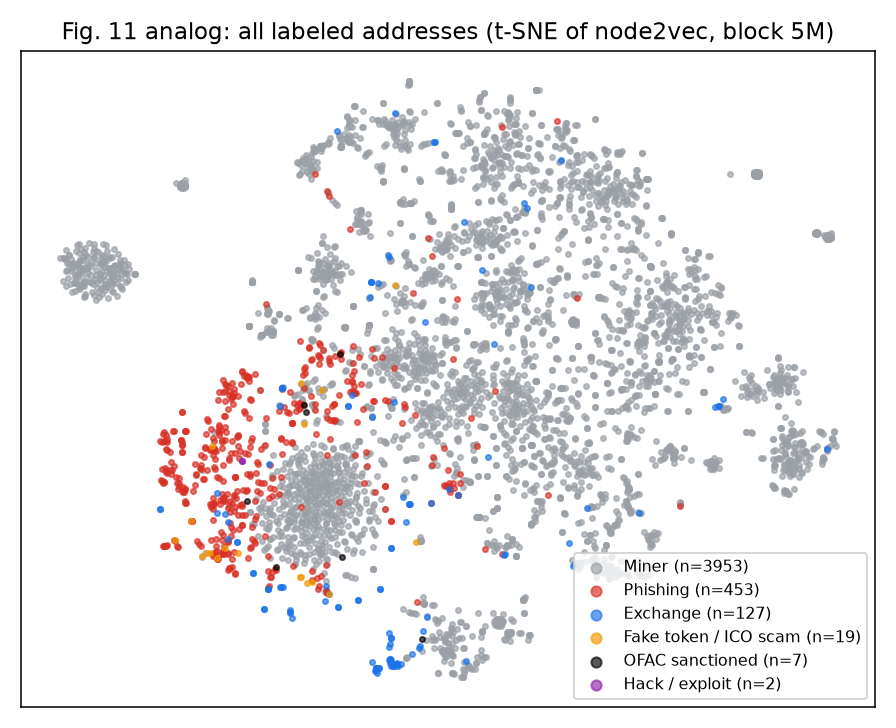
\includegraphics[width=0.66\textwidth]{figures/tsne_all}
\caption{Analog of the paper's Figure~11: t-SNE \cite{tsne} of dynamic node2vec embeddings (block 5\,M) for all labeled addresses. Phishing addresses (red) occupy a distinct region; miners (grey) cover most of the rest; exchanges (blue) are scattered.}
\label{fig:tsne_all}
\end{figure}
\begin{figure}[H]
\centering
\begin{subfigure}{0.48\textwidth}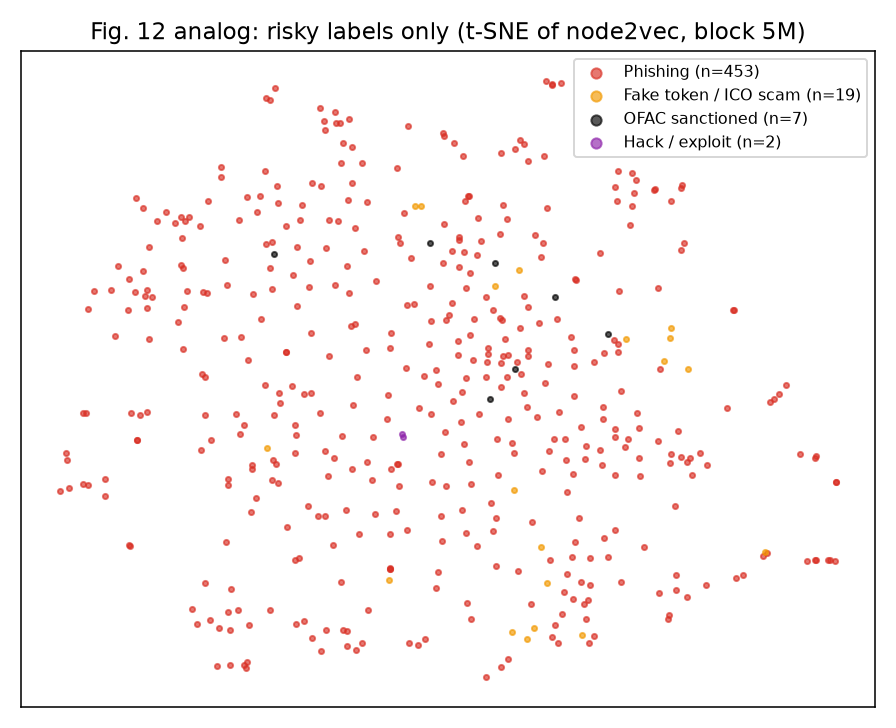
\includegraphics[width=\textwidth]{figures/tsne_risky}\caption{Risky labels only.}\end{subfigure}\hfill
\begin{subfigure}{0.48\textwidth}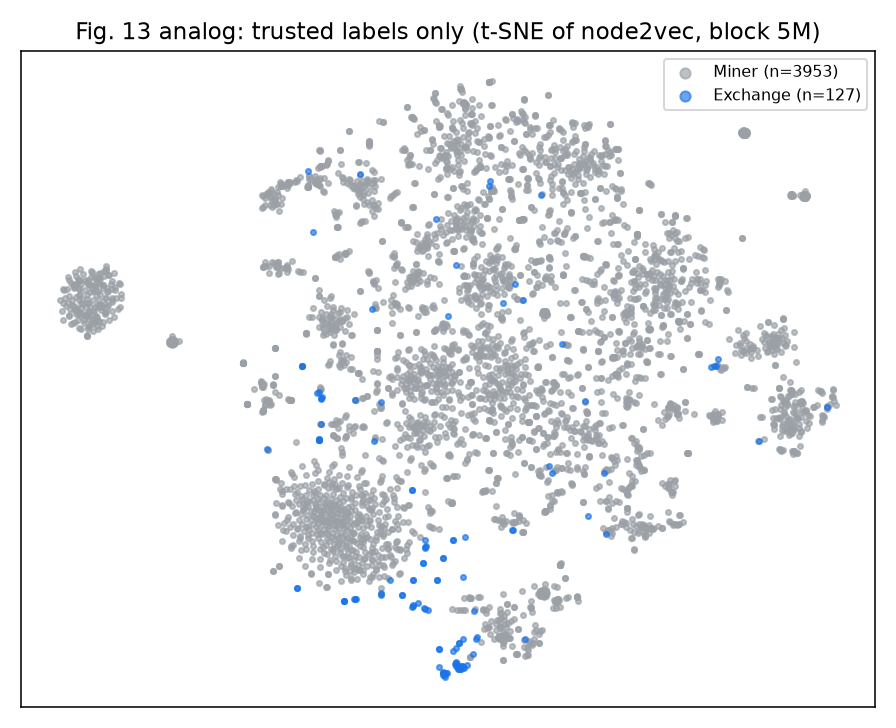
\includegraphics[width=\textwidth]{figures/tsne_trusted}\caption{Trusted labels only.}\end{subfigure}
\caption{Analogs of the paper's Figures~12 and~13, each projected separately.}
\label{fig:tsne_sub}
\end{figure}
``Visible clusters'' is a subjective criterion, so Table~\ref{tab:tsne} adds objective measures computed in the original 128-dimensional space, each next to a control with shuffled labels.
\begin{table}[H]
\centering\footnotesize\singlespacing
\begin{tabular}{l r cc cc c}
\toprule
 & $n$ & \multicolumn{2}{c}{silhouette (cosine)} & \multicolumn{2}{c}{5-NN accuracy} & majority\\
\cmidrule(lr){3-4}\cmidrule(lr){5-6}
 & & real & shuffled & real & shuffled & baseline\\
\midrule
Bad vs.\ good (all labeled) & 4,561 & 0.242 & -0.001 & 0.953 & 0.887 & 0.895\\
Six groups (Fig.~11 analog) & 4,559 & 0.011 & -0.070 & 0.938 & 0.857 & 0.867\\
Risky sub-types only (Fig.~12) & 479 & -0.148 & -0.068 & 0.948 & 0.946 & 0.942\\
Miners vs.\ exchanges (Fig.~13) & 4,080 & 0.457 & -0.014 & 0.979 & 0.969 & 0.969\\
\bottomrule
\end{tabular}
\caption{Cluster separation of the embeddings. Silhouette near 0 means no structure; 5-NN accuracy is 5-fold cross-validated and should be compared with the majority-class baseline.}
\label{tab:tsne}
\end{table}
The embedding separates the risk classes: bad versus good has a 5-NN accuracy of \TsneBadGoodKnn{} (balanced accuracy \TsneBadGoodBal) against a majority baseline of 0.895, and a silhouette of \TsneBadGoodSil{} (shuffled labels: about 0). Miners and exchanges also separate (silhouette 0.457). Finer sub-types of risky addresses (fake-token scams, hacks, OFAC) do not separate beyond the baseline, but these classes are tiny (19, 2 and 7 addresses) and noisily tagged, so no conclusion is possible for them.

\section{Scorecard and Analysis}
\label{sec:scorecard}
\begin{table}[H]
\centering\footnotesize\singlespacing
\begin{tabular}{p{3.7cm} p{3.0cm} p{5.3cm} p{1.8cm}}
\toprule
\textbf{Paper's claim} & \textbf{Paper} & \textbf{Our evidence} & \textbf{Verdict}\\
\midrule
Combining graph and behavioural features beats either alone (Table~II) & F$_1$ 0.851 vs.\ 0.738 / 0.718 & Gain +0.008 (A) / +0.004 (B), within noise; clean covered-only subset: 0.942 vs.\ 0.952 for behaviour alone & \vNo\\
Graph features beat behavioural features alone & 0.738 vs.\ 0.718 (gap 0.02, no CI) & Reversed: 0.871 (A), 0.753 (B) vs.\ 0.956 & \vNo\\
Dynamic node2vec beats propagation (Table~IV) & Gap 0.13--0.19 AUC at all checkpoints & Higher at all three checkpoints (+0.103, +0.037, +0.085 PR-AUC); clear only at 5.0\,M; full coverage vs.\ 79--89\% & \vPart\\
Best setting is 10 walks, length 10, $p=q=1$; more walks help (Table~III) & Best 0.814; walks 0.751 $\to$ 0.795 & Best \BestPRAUC{}; walks 0.865 $\to$ 0.929; $p,q$ effects within noise & \vOK\\
Propagation reaches about 78\% of addresses & 78\% (80--85\% of daily-active) & \CovA\% (A) and \CovB\% (B) on the whole graph; 98--100\% in our universe & \vPart\\
Embeddings show label clusters (Figs.\ 11--13) & Qualitative & Bad vs.\ good separable (5-NN \TsneBadGoodKnn{} vs.\ 0.895 baseline); sub-types not separable (tiny classes) & \vPart\\
Node2vec has high feature importance & Stated, not shown & 56.3\% (A), 46.7\% (B), biased by column count & \vPart\\
Scales to every address and updates incrementally & Deployed at 266\,M & Demonstrated on a 3\,M-node universe (checkpoint updates, bit-identical distributed walks); not tested at paper scale & untestable here\\
\bottomrule
\end{tabular}
\caption{Scorecard. ``Reproduced'' means the ordering or trend holds on our data, not that absolute numbers match.}
\label{tab:scorecard}
\end{table}

\subsection{Why do the headline claims differ?}
We rank explanations by how well our evidence supports them.
\begin{enumerate}
\item \textbf{Ceiling effect from an easy negative class (well supported).} Behavioural features alone reach F$_1$ 0.956, and with exchanges as the only negatives every feature set in variant A saturates at 0.98--0.99. When behaviour already separates the classes, there is little for graph embeddings to add. The paper's much lower behavioural score (0.718) leaves room for the complementary gain it reports.
\item \textbf{Different negative class (plausible).} Our negatives are miners and exchanges; the paper's include government addresses and, plausibly, a broader mix. We cannot verify this because its labels are private.
\item \textbf{Label noise and era mismatch (plausible, unmeasured).} Our labels are a 2022 snapshot of Etherscan tags applied to 2015--2018 activity, and labeled bad addresses may have been well known and structurally distinctive; the paper's labels come largely from curated internal sources plus undisclosed external ones.
\item \textbf{Scale (plausible).} Neighbourhood structure in a graph 11 times smaller and five years earlier may carry less signal. The coverage numbers show the geometry differs.
\item \textbf{Embedding quality at fixed budget (possible).} We trained one epoch at dimension 128 with unspecified skip-gram settings. Better-tuned embeddings could narrow the gap, but our sweep shows large gains from more walks, which suggests the node2vec features are not yet saturated; a longer training would be a cheap check.
\end{enumerate}

\subsection{What we can and cannot conclude}
We can conclude that the paper's \emph{engineering} claims hold up in direction: node2vec settings, the benefit of incremental embedding over propagation (with full coverage), and the practicality of a streaming, partitioned pipeline. We cannot confirm or refute its headline ablation, because our data differ in exactly the ways that would hide or reverse such an effect. We did \emph{not} find evidence that the paper is wrong; we found that the claim is fragile to the negative class.

\subsection{Threats to validity}
\begin{itemize}
\item \textbf{Single training run per method} in Tables~II and IV. The reported intervals reflect random train/test splits of fixed embeddings, not retraining variation, which we measured at about 0.01 PR-AUC. Part of the Table~IV gap could be training noise.
\item \textbf{Small bad class}, 481 addresses in total and 34 at the first checkpoint, makes some rows noisy.
\item \textbf{No external test set or temporal split.} Train and test addresses come from the same pool, as in the paper; a time-ordered split would be stricter.
\item \textbf{Label provenance} (Etherscan-derived) carries selection bias and a terms-of-use caveat.
\item \textbf{Multiple comparisons.} We inspected many configurations; the noise band guards against over-reading, but isolated differences should not be treated as findings.
\item \textbf{Unweighted snapshots, a 3\,M-node universe and a core that is a third of it} in Table~IV differ from the paper's larger core share relative to its universe.
\end{itemize}

\subsection{Inconsistencies and gaps found in the paper}
We list these neutrally; none changes our conclusions but each made reproduction harder.
\begin{enumerate}
\item The behavioural features are said to be ``defined in Table~1'', but Table~I is the data-source table; the feature list is never given.
\item The text says the hyperparameter AUC values are in ``Table~II''; they are in Table~III. Table~II is the feature-set comparison.
\item Table~III has blank cells (for example length~4, $p=0.25$ and $q=0.25$ rows).
\item The captions of Figures~8 and~9 appear swapped: Figure~8 is titled ``In-out Parameter (p)'' and Figure~9 ``Return parameter (q)''.
\item The graph size is given as about 266\,M addresses in the introduction and about 275\,M in the conclusion.
\item The dynamic-node2vec citation points to reference~[2], an unrelated paper on money laundering (dynnode2vec is reference~[11]), and the MapReduce citation points to reference~[3], also unrelated.
\item References [12] and [14] are the same paper listed with different years.
\item The hardware section mentions CPUs, PyTorch and ``GNN models'', although the system uses node2vec with gensim, and a footnote describes a V100 GPU.
\item The incremental step is described as ``daily'' while checkpoints are millions of blocks apart (about 830 daily steps from 10\,M to 16\,M); the actual step size is unclear.
\item The metric called ``AUC'' in Tables~III and~IV is not defined; Table~II's classification threshold is not stated; no uncertainty is reported anywhere.
\item Minor: the organisation paragraph refers to Section~6 for the conclusion (it is Section~V); ``Propogation'' is misspelled in an algorithm title.
\end{enumerate}

% =====================================================================================================
\section*{Part B: CryptoTrace}
\addcontentsline{toc}{section}{Part B: CryptoTrace}

\section{Evaluation Set-up}
\label{sec:evalsetup}
CryptoTrace was run on three cases (Table~\ref{tab:cases}). Two are documented hacks, taken from the textbook's case studies, whose published answers say where the funds went. The third is a real wallet that Etherscan users tagged as phishing; it has \emph{no} published answer, and it was selected from the public labels because its trace reaches exchange deposit addresses. That selection bias is disclosed in the application, in this report and in the case description. Each case was traced with three strategies: TTR-lite, Haircut taint and blind BFS (depth 2), with the default parameters of Table~\ref{tab:datamodel}.

\begin{table}[H]
\centering\small\singlespacing
\begin{tabular}{p{3.2cm} p{3.0cm} p{2.6cm} p{4.2cm}}
\toprule
\textbf{Case} & \textbf{Window} & \textbf{Funds leaving source} & \textbf{Published answer}\\
\midrule
Cryptopia exchange hack (May 2019) & 2019-05-14 to 2019-06-28 & 30\,766 ETH & EtherDelta within two hops; later Yobit.net and OKEx\\
KuCoin exchange hack (Sept.\ 2020) & 2020-09-25 to 2020-11-10 & 11\,533 ETH & About 13.8K ETH into the Tornado Cash 100 ETH pool\\
Phishing-labeled wallet (2018) & 2018-06-29 to 2018-08-13 & 2\,450 ETH & None (selected by us; label Fake\_Phishing1951)\\
\bottomrule
\end{tabular}
\caption{The three cases. Source addresses: Cryptopia \code{0xd4e79226\dots8d11}; KuCoin \code{0xeb31973e\dots8c23}; phishing \code{0x5457bb44\dots5b9b}.}
\label{tab:cases}
\end{table}

\section{Case 1: KuCoin Exchange Hack (September 2020)}
The hacker's wallet received ETH from KuCoin and moved most of it into Tornado Cash. TTR-lite reaches the Tornado Cash 100 ETH pool in two hops: 99.8\% of the funds, about 11\,511 ETH (Table~\ref{tab:dest_kucoin}). The evidence path has two transfers (Table~\ref{tab:path_kucoin}): 11\,500 ETH from the reported wallet to an intermediate address on 2020-10-23 at 07:40 UTC, then 100 ETH on to the pool at 08:06 UTC. The trace stops there because a mixer breaks the on-chain link; the destination is a high-confidence stop and the interface says that tracing cannot continue by this method. The published figure is about 13.8K ETH; ours is lower because of our window and the 0.01 ETH dust filter.

\gentable{gen/tab_dest_kucoin_2020.tex}{Destinations found for the KuCoin case (TTR-lite).}{tab:dest_kucoin}
\gentable{gen/tab_path_kucoin_2020.tex}{Evidence path to the Tornado Cash pool.}{tab:path_kucoin}
\gentable{gen/tab_rounds_kucoin_2020.tex}{Search rounds for the KuCoin case: accounts expanded, destinations absorbed and the share of funds still unexplained.}{tab:rounds_kucoin}

\shot{27_lab_kucoin_round1}{Trace Lab, KuCoin case, early in the search. The reported wallet and the first intermediate account appear; 85\% of the funds are still unexplained.}
\shot{28_lab_kucoin_final}{Trace Lab, KuCoin case, finished. The headline sentence states that 99.8\% of the traced funds reached Tornado Cash and that tracing stops at a mixer.}
\shot{29_lab_kucoin_mixer_expanded}{KuCoin case with the finding expanded: a high-confidence mixer stop, the two-transfer evidence path with transaction links, and the laundering pattern seen (one fast hop).}

\section{Case 2: Cryptopia Exchange Hack (May 2019)}
About 30.8K ETH was stolen from the Cryptopia exchange. TTR-lite follows 99.98\% of it (about 30\,760 ETH) to a single address in 500--1\,000 ETH batches, within six rounds; that address is the EtherDelta DEX contract (Table~\ref{tab:dest_cryptopia}). The curated label for EtherDelta is marked \emph{unverified on-chain}, so the finding carries medium confidence. The highest-value evidence path has five transfers (Table~\ref{tab:path_cryptopia}), and the shortest route to the contract is two hops. The share of unexplained funds falls more slowly than in the other cases (Table~\ref{tab:rounds_cryptopia}) because the funds move through a chain of intermediate accounts. The textbook reports that the funds later left through Yobit.net and OKEx; \emph{we do not reach these}, because they sit behind the DEX contract and the exit from a contract is an internal transfer, which the external-transfer data we use does not contain. We therefore record this case as one of three expected destinations reached (EtherDelta yes; Yobit.net and OKEx not reached) and list DEX pass-through as the first item of the pending work.

\gentable{gen/tab_dest_cryptopia_2019.tex}{Destinations found for the Cryptopia case (TTR-lite).}{tab:dest_cryptopia}
\gentable{gen/tab_path_cryptopia_2019.tex}{Evidence path to the EtherDelta contract (highest-value route).}{tab:path_cryptopia}
\gentable{gen/tab_rounds_cryptopia_2019.tex}{Search rounds for the Cryptopia case.}{tab:rounds_cryptopia}

\shot{30_lab_cryptopia_mid}{Trace Lab, Cryptopia case, mid-search (round 2 of 6): eight accounts, 72\% unexplained.}
\shot{31_lab_cryptopia_final}{Trace Lab, Cryptopia case, finished: 100\% of the traced funds (about 30\,760 ETH) reached the EtherDelta DEX contract; the note says that the way out is an internal transfer this prototype cannot yet follow.}
\shot{32_lab_cryptopia_dex_expanded}{Cryptopia finding expanded: medium confidence, ``labeled dex (curated; unverified on-chain)'', and the five-transfer evidence path. In total 18 transfers from the traced accounts entered the contract, about 9\,502 ETH of them visible within the window and the 200-transfer cap.}
\shot{33_lab_cryptopia_bfs_final}{Cryptopia traced by blind BFS: it also reaches the contract but attributes only 4.3\% of the funds to it, because it stops after two hops and splits shares uniformly.}

\section{Case 3: Phishing-Labeled Wallet (2018)}
\label{sec:phish}
This is the main demonstration case. A wallet that Etherscan users tagged as phishing sent about 2\,450 ETH between June and August 2018. TTR-lite finishes in five rounds touching 75 accounts and 1\,390 transfers (Table~\ref{tab:rounds_phish}); BigQuery was not queried at run time because the case was already cached. The results are:
\begin{itemize}
\item \textbf{90.9\% of the funds, about 2\,227 ETH, reached 29 distinct deposit addresses} that each forward their outflow to the labeled exchange wallet \emph{ShapeShift 3} (the sweep rule), within two hops. These are inferred deposit addresses with medium confidence (Table~\ref{tab:dest_phish}, Figure~\ref{fig:deposit_share}).
\item \textbf{5.2\%, about 128 ETH, reached two unlabeled high-activity services} (one with 10\,512 and one with 17\,869 transfers in the window), where the trace stops with low confidence and a manual-review flag (Table~\ref{tab:hubs}).
\item The funds first move in one transfer of 2\,198 ETH to an intermediate account on 2018-07-11, which splits them mainly into 100 ETH pieces. The highest-value evidence path to a deposit address has three transfers (Table~\ref{tab:path_phish_top}): 2\,198 ETH, then 101 ETH, then 10.2 ETH, ending at the deposit address \code{0x5ea511\dots04f1} on 2018-07-19.
\item The typology engine tags 26 accounts as zero-out (forwarding almost everything within a day) and 27 as fast hops (Table~\ref{tab:tags}).
\end{itemize}

\gentable{gen/tab_dest_phishing_2018.tex}{Destinations found for the phishing case (TTR-lite). Twenty-nine deposit addresses are grouped into one finding.}{tab:dest_phish}
\gentable{gen/tab_rounds_phishing_2018.tex}{Search rounds for the phishing case.}{tab:rounds_phish}
\gentable{gen/tab_hubs.tex}{The two unlabeled high-activity services where the phishing trace stops.}{tab:hubs}

\begin{figure}[H]
\centering
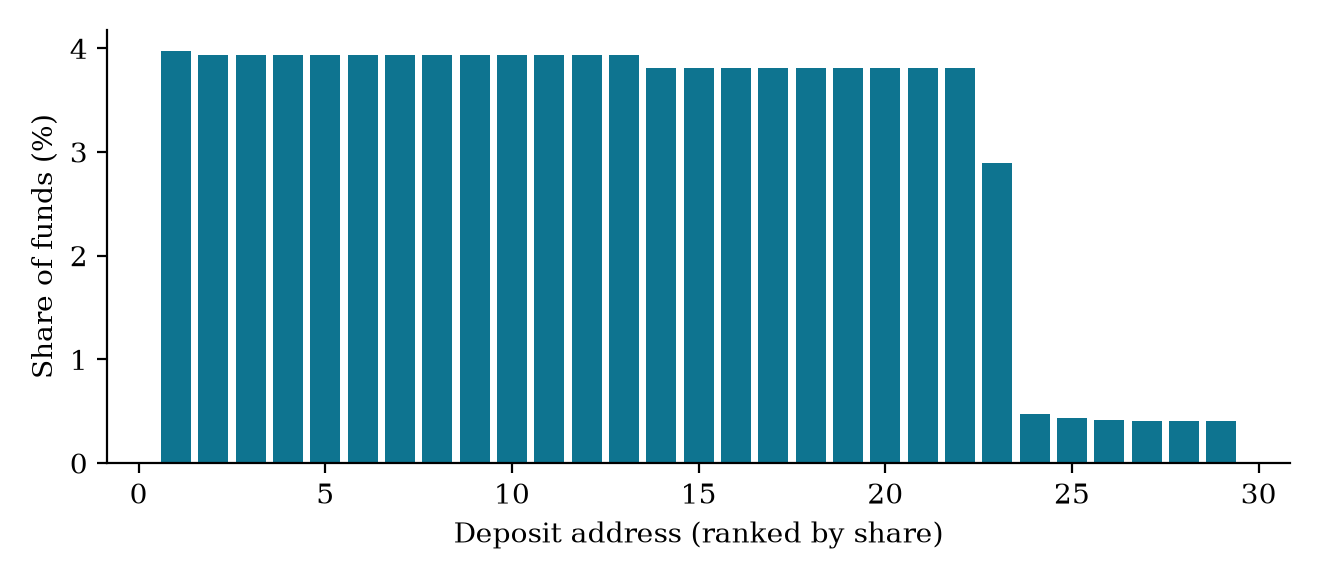
\includegraphics[width=0.9\textwidth]{figs/deposit_share.png}
\caption{Share of the funds reaching each of the 29 deposit addresses, ranked. Twenty-two addresses receive about 3.8--4.0\% each, which matches the splitting of the funds into near-equal pieces; the last six receive about 0.4\% each.}
\label{fig:deposit_share}
\end{figure}

\begin{figure}[H]
\centering
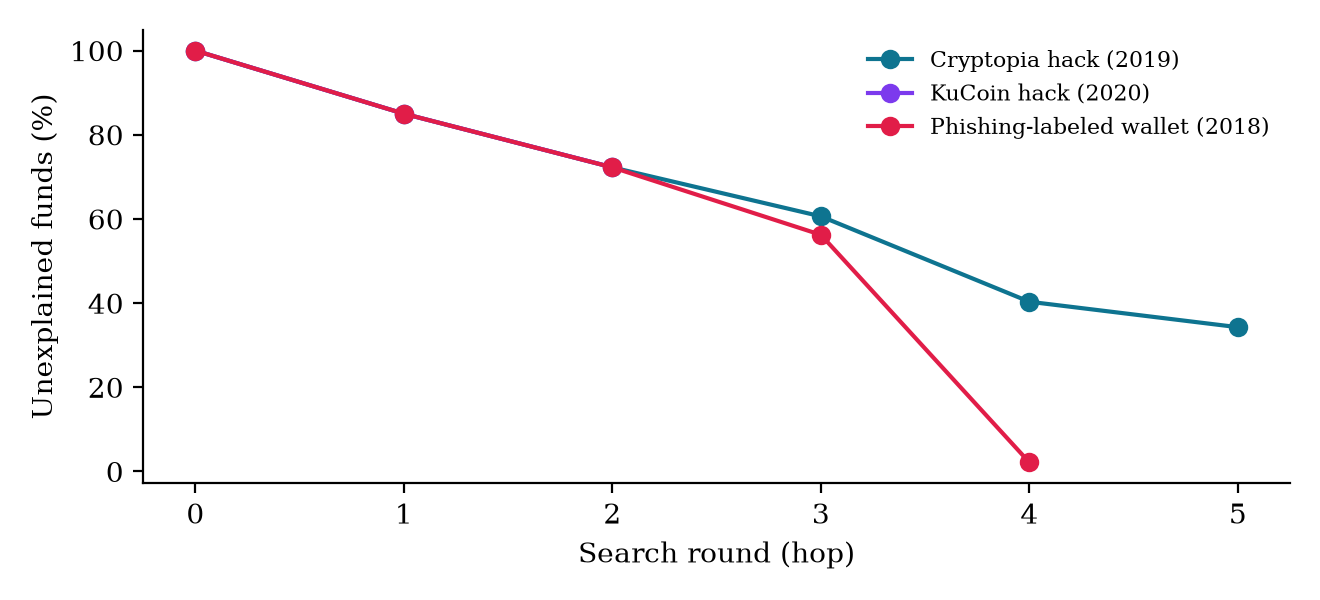
\includegraphics[width=0.9\textwidth]{figs/residual_decay.png}
\caption{Unexplained funds after each search round for the three cases. The phishing case drops from 56\% to 2\% in round 4, when the deposit addresses are reached; the Cryptopia case declines more slowly because the funds pass through a chain of accounts.}
\label{fig:residual_decay}
\end{figure}

\subsection{Stepping through the search}
Figures~\ref{fig:13_lab_phishing_start} to~\ref{fig:17_lab_phishing_final} show the same trace at successive rounds, exactly as the application plays it. At round 0 only the reported wallet exists. In round 1 the search fetches its neighbourhood (one cached lookup) and finds the first recipient. By round 2 the 100 ETH pieces appear. In round 3 the frontier grows to 32 accounts and the first deposit addresses are absorbed, and in round 4 the remaining funds are explained and 2\% remain unexplained, at which point the search ends.

\shot{13_lab_phishing_start}{Phishing case, round 0: only the reported wallet. The result column already shows the stored finding; the data-layer counter reads 0 queries, 0 cached.}
\shot{14_lab_phishing_round1}{Round 1: four accounts and four transfers; 85\% of the funds are unexplained; one cached lookup.}
\shot{15_lab_phishing_round2}{Round 2: 29 accounts and 29 transfers; 72\% unexplained. The hub that splits the funds appears.}
\shot{16_lab_phishing_round3}{Round 3: 44 accounts; 56\% unexplained; 37 cached lookups. The first deposit addresses are absorbed (teal rings).}
\shot{17_lab_phishing_final}{Round 4: 2\% unexplained, 63 cached lookups, no queries. The top finding is highlighted automatically when playback ends, and its deposit address is labeled on the canvas.}

\subsection{Reading the finding}
The finding card (Figure~\ref{fig:18_lab_phishing_group_expanded}) states the entity (ShapeShift 3), the number of addresses (29), the share and amount (90.9\%, about 2\,227 ETH), the confidence (medium), the type (exchange deposit, inferred) and the rule that produced it (``forwards 100\% of its outflow to ShapeShift 3 within 48 h''). Below it is the list of addresses to ask the exchange to freeze, with each address's share and amount, and the evidence path to the largest of them (Figure~\ref{fig:19_lab_phishing_paths}), each transfer with its amount, time and a link to the transaction on a public block explorer.

\shot{18_lab_phishing_group_expanded}{The grouped finding expanded: ShapeShift 3, 29 addresses, medium confidence, the sweep rule, and the addresses to ask the exchange to freeze.}
\shot{19_lab_phishing_paths}{Evidence path to the largest deposit address (three transfers with timestamps and transaction links), and a statement of how many transfers in total entered these addresses (287, about 2\,308 ETH).}

\gentable{gen/tab_path_phishing_2018.tex}{Evidence path recorded in the case file for the first service account on the phishing trace (the hub reached through the 100 ETH piece).}{tab:path_phish_hub}
\begin{table}[H]
\centering\small\singlespacing
\begin{tabular}{r p{2.9cm} p{2.9cm} r p{2.5cm}}
\toprule
\textbf{\#} & \textbf{From} & \textbf{To} & \textbf{ETH} & \textbf{Time (UTC)}\\\midrule
1 & \texttt{0x5457bb..7c5b9b} & \texttt{0x5979e2..0c6f14} & 2\,198.39 & 2018-07-11 21:05\\
\multicolumn{5}{l}{\quad tx: \texttt{\scriptsize 0x445f791d730719386f01a56ca2d5dd78d85604a1581d0f636116d4c585122485}}\\
2 & \texttt{0x5979e2..0c6f14} & \texttt{0x76fc36..f646a0} & 101.14 & 2018-07-19 13:32\\
\multicolumn{5}{l}{\quad tx: \texttt{\scriptsize 0x9d81bd959bee5cf670e0f3b113c77abd41714dc6567a8e2cbc7da2922c364ad1}}\\
3 & \texttt{0x76fc36..f646a0} & \texttt{0x5ea511..04f1} & 10.20 & 2018-07-19 14:19\\
\multicolumn{5}{l}{\quad tx: \texttt{\scriptsize 0x027926853601d26e17fecfd23ac3206ff8e79b4934a6cbb5399534d63eb8a904}}\\
\bottomrule\end{tabular}
\caption{Evidence path to the largest deposit address (3.98\% of the funds), from the case file.}
\label{tab:path_phish_top}
\end{table}

\subsection{Inside the engine, and a single account}
The \emph{Inside the engine} tab (Figure~\ref{fig:20_lab_phishing_engine_tab}) narrates what the engine did in the current round: the frontier size, the weights of the highest-residual accounts, the unexplained funds per round as a small chart, and the list of stops with the rule that triggered each. The \emph{Account} tab (Figure~\ref{fig:21_lab_phishing_account_tab}) describes a clicked account: its address with a link to the explorer, role, label, share of funds, hops from the source, time of first funds, transfers in and out within the window, and its rank.

\shot{20_lab_phishing_engine_tab}{The \emph{Inside the engine} tab: each stop is listed with the sweep rule that triggered it.}
\shot{21_lab_phishing_account_tab}{The \emph{Account} tab for the deposit address \code{0x5ea511\dots04f1}: role exchange deposit (inferred), 3.98\% of funds, three hops, first funds 2018-07-19 13:44 UTC, 12 transfers in and 2 out.}
\shot{22_lab_parameters_panel}{The result column scrolled to show the second finding (two unlabeled high-activity services, low confidence), the laundering patterns seen (zero-out 26, fast hop 27) and the limits of the prototype; the control column shows the parameter sliders and the Run trace button.}

\gentable{gen/tab_tags.tex}{Laundering-pattern tags per case (number of accounts tagged, TTR-lite).}{tab:tags}

\section{Comparison of the Three Strategies}
Table~\ref{tab:runs} lists every run. On the two documented hacks all three strategies reach the published destination, but with different effort and different attribution of the funds. On the phishing case the strategies separate: TTR-lite and Haircut taint each reach 31 destinations (29 deposit addresses and two hubs), while blind depth-2 BFS reaches none, because the funds only arrive at deposit addresses after the third hop and the BFS stops after the second.

\gentable{gen/tab_runs.tex}{All nine runs: rounds, accounts in the result graph, transfers considered, depth, destinations reached and the top destination with its share.}{tab:runs}

\begin{figure}[H]
\centering
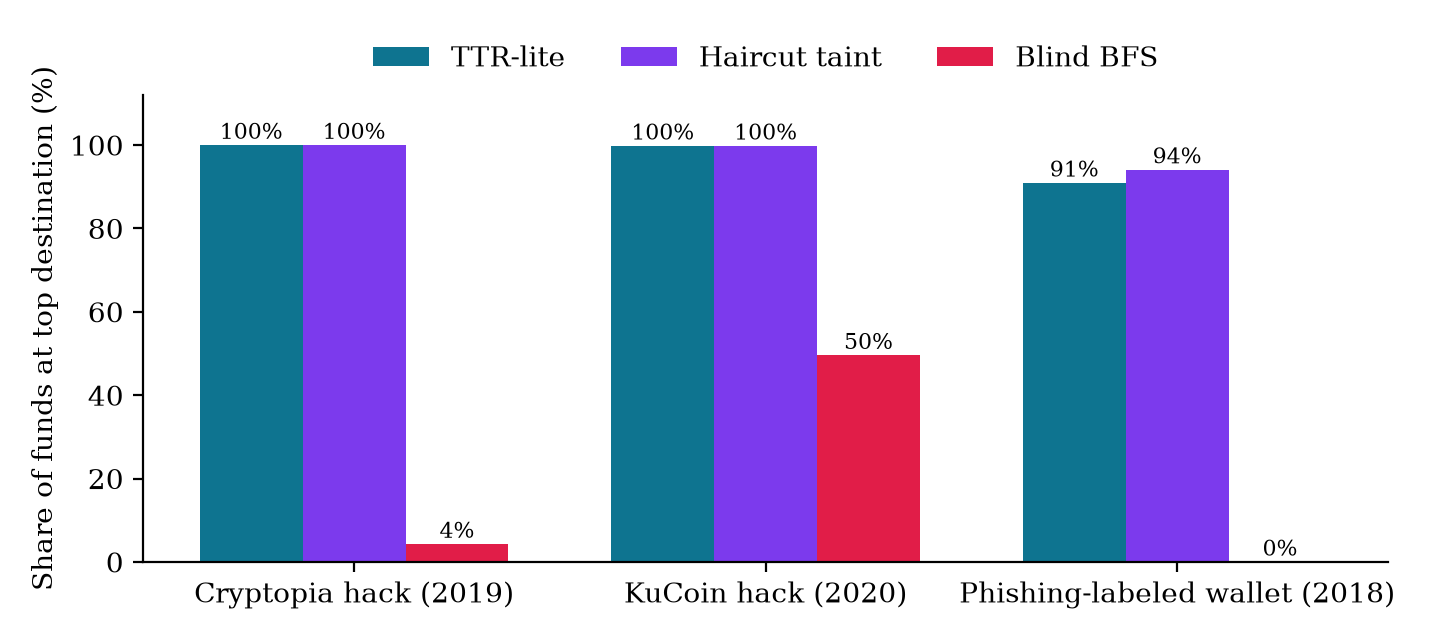
\includegraphics[width=0.95\textwidth]{figs/share_by_engine.png}
\caption{Share of the funds attributed to the top destination, by case and strategy. BFS attributes only 4\% (Cryptopia) and 50\% (KuCoin) of the funds to the correct destination and 0\% on the phishing case.}
\label{fig:share_by_engine}
\end{figure}
\begin{figure}[H]
\centering
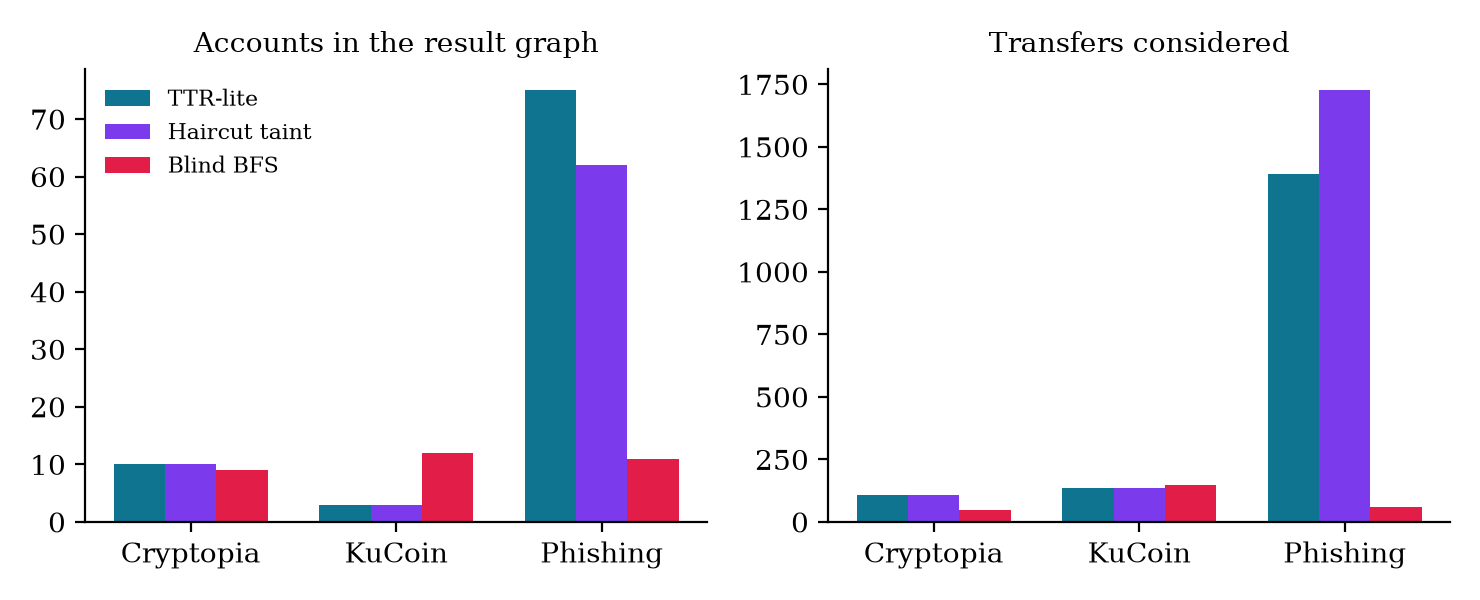
\includegraphics[width=0.98\textwidth]{figs/effort_by_engine.png}
\caption{Effort by strategy: accounts in the result graph (left) and transfers considered (right).}
\label{fig:effort}
\end{figure}

\paragraph{Observations.}
\begin{itemize}
\item \emph{Ranked and taint searches agree closely.} On KuCoin and Cryptopia their results are identical; on the phishing case they differ slightly (90.9\% against 94.1\% attributed to ShapeShift 3; 75 against 62 accounts; five against seven rounds). TTR-lite also follows a small share backwards, which adds upstream accounts to the graph.
\item \emph{BFS fails in two different ways.} It reaches no destination at all on the phishing case, and on the two hacks it reaches the right destination but attributes only a fraction of the funds to it (4.3\% and 49.6\%), since it spreads shares uniformly across every neighbour.
\item \emph{BFS is not reliably cheaper.} On the Cryptopia and phishing cases it considers far fewer transfers than the ranked search (48 against 106, and 59 against 1\,390), which is exactly why it stops short; on KuCoin it considers slightly more (146 against 135) and returns more accounts (12 against 3) for an investigator to review.
\item \emph{This separation matches the published benchmark in kind.} The textbook's 20-case table (Table~\ref{tab:bookbench}) shows blind BFS reviewing about 52\,500 accounts for 77\% recall and the ranked search about 870 for 92\%. Our three cases are too few to say anything about numbers, only about direction.
\end{itemize}

\shot{24_lab_phishing_haircut_final}{Phishing case with the Haircut strategy: the same destination with 94.1\% of the funds, seven rounds.}
\shot{25_lab_phishing_bfs_final}{Phishing case with blind BFS: the search ends after two hops without reaching any labeled destination, and the interface explains why.}

\section{What-If Re-Runs at Zero Cost}
Because every neighbourhood is cached, parameters can be changed and the trace re-run at once with no BigQuery cost. Figure~\ref{fig:26_lab_whatif_3rounds} shows the phishing case re-run with the maximum number of rounds lowered to three. The search stops at the hop limit and the interface warns that unexplored flows remain; 56\% of the funds are still unexplained, only 5 of the 29 deposit addresses have been reached (about 4.5\% of the funds, roughly 108 ETH), the unlabeled hub holds 4.1\% (about 100 ETH), and the data-layer counter shows 37 cached lookups and no queries. This is how a presenter can show the algorithm responding to its settings without waiting.

\shot{26_lab_whatif_3rounds}{What-if re-run with the round limit lowered to 3: the search stops early, a warning says unexplored flows remain, and the unexplained share stays at 56\%.}

\section{BigQuery Cost}
Table~\ref{tab:cost} and Figure~\ref{fig:bq_cost} summarise the cost of first fetches. A per-hop query returns only the largest transfers per address, but BigQuery bills by the partitions scanned for the time window, so the cost depends on the window and not on the number of addresses in a chunk. Each case therefore cost cents, and all later runs were free.

\begin{table}[H]
\centering\small\singlespacing
\begin{tabular}{p{5.2cm} r r}
\toprule
\textbf{Item} & \textbf{Scanned (GiB)} & \textbf{List-price cost (USD)}\\
\midrule
Reproduction extraction (blocks 0--5\,M, Tier S) & 48.6 & about 0.30\\
Cryptopia case, first fetch & 9.51 & about 0.06\\
KuCoin case, first fetch & 3.87 & about 0.02\\
Phishing case, first fetch & 19.90 & about 0.12\\
Exploration query used to find the phishing example & 29.9 & about 0.18\\
\bottomrule
\end{tabular}
\caption{BigQuery scanning at an assumed list price of \$6.25 per TiB (to be checked against current pricing; the first TiB each month is free). Total for the tracing prototype, including other exploration, is roughly \$0.6.}
\label{tab:cost}
\end{table}
\begin{figure}[H]
\centering
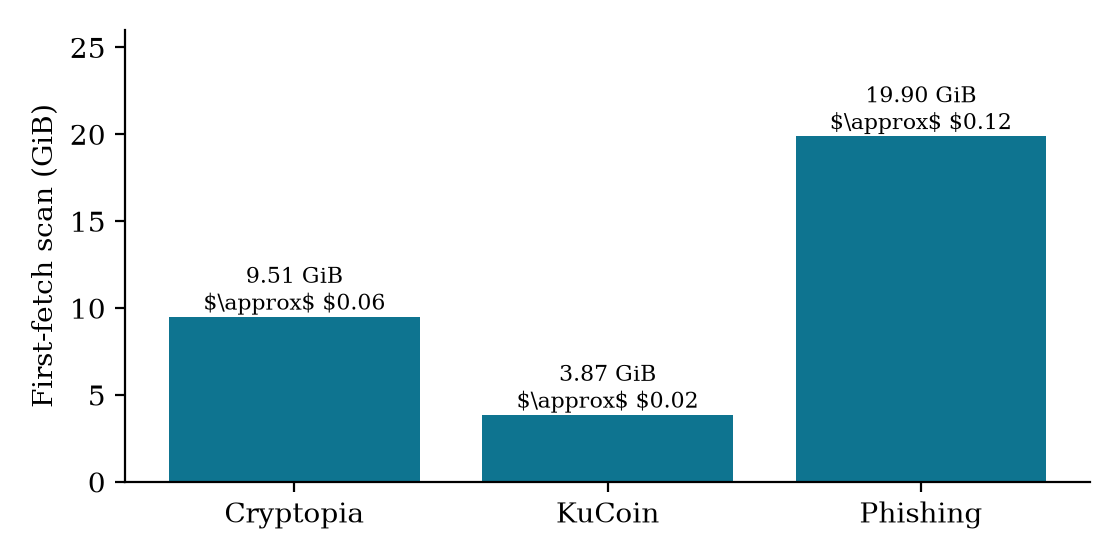
\includegraphics[width=0.7\textwidth]{figs/bq_cost.png}
\caption{First-fetch scan size and approximate cost per case.}
\label{fig:bq_cost}
\end{figure}

\section{A Walk through Every Screen}
\label{sec:screens}
This section shows every screen of the application. All screenshots were taken by a script (\code{scripts/ct\_screenshots.mjs}) that drives a real browser against the running application at a 1440$\times$900 viewport at 1.5$\times$ resolution, selecting the case, strategy and search round explicitly for each image. Full-page captures are in Appendix~\ref{app:screens}.

\subsection{Overview}
The Overview page (Figure~\ref{fig:01_overview_top}) states the problem in one sentence and gives four headline figures: 100\% of the Cryptopia funds followed to the EtherDelta DEX in six rounds; 99.8\% of the KuCoin funds followed into the Tornado Cash pool in three rounds, where tracing correctly stops; the cost of the first full Cryptopia trace (about \$0.06); and ``29 $\to$ 1'', the number of deposit addresses traced from one phishing-labeled wallet into a single exchange. Below are the four steps of a trace (report a wallet, follow the money, stop at a service, hand over evidence) and the three cases, each with its headline result, number of rounds, accounts in the graph and first-fetch size. A closing box states what the prototype is and is not.

\shot{01_overview_top}{Overview page: headline figures, how a trace works, and the cases.}
\shotw{44_overview_tablet}{The Overview page at tablet width (820 px): the cards reflow into two columns.}{0.5}

\subsection{System}
The System page (Figure~\ref{fig:03_system_idle}) draws the architecture of Chapter~\ref{ch:design} from the module data: five columns (intake, data layer, engines, output, evaluation), each module with its status (live, partial or planned), a switch to hide the planned modules, and dashed arrows for data flow. Clicking a module opens its details: what it does, what is live and what is pending, which problem-statement requirements it serves. The button \emph{Play a trace through the system} replays a real trace through the modules (Figures~\ref{fig:05_system_playing} and~\ref{fig:06_system_playing_late}): the intake opens the case, the adapter fetches, the cache reports its first-fetch size, the tracing engine reports each round and the share of funds still unexplained, the attribution engine states where it stops, the typology engine counts the patterns, and the case file and report are written. A log on the page narrates each step with the numbers of the case.

\shot{03_system_idle}{System page at rest: status badges, the planned modules shown dashed, and the data-flow arrows.}
\shot{05_system_playing}{System page while a trace plays through the modules (the tracing engine is lit).}
\shot{06_system_playing_late}{Later in the same playback: the investigator report is lit.}

\subsection{Trace Lab}
The Trace Lab is the centre of the application and has been shown above case by case. Its three columns are the \emph{controls} (demo guide, case picker with the case's story, strategy buttons with a one-line description of each strategy, parameter sliders for $\alpha$, $\beta$, $\epsilon$, maximum rounds and hub threshold, a time-respecting switch and a Run button), the \emph{graph} with a heads-up display (round, accounts, transfers, unexplained share, data layer), a legend and a playback bar (back, play or replay, forward, scrubber, speed, fit), and the \emph{result column} with the tabs Findings, Inside the engine and Account. The case picker can be switched to \emph{Any wallet} (Figures~\ref{fig:34_lab_anywallet_empty} and~\ref{fig:35_lab_anywallet_cache_miss}): the user enters an address and dates; live BigQuery access is a switch that is off unless the server was started with credentials, so an address that was never fetched ends with a clear message instead of a bill.

\shot{34_lab_anywallet_empty}{The \emph{Any wallet} mode of the case picker (the previous result is still shown until a new run starts).}
\shot{35_lab_anywallet_cache_miss}{A custom address that was never fetched: ``1 address(es) are not cached for this window; enable live BigQuery to fetch them''. Nothing is billed.}
\shotw{23_lab_phishing_1280x720}{The Trace Lab at 1280$\times$720, the projector size: the three columns fit without scrolling the page.}{0.85}

\subsection{Compare}
The Compare page (Figures~\ref{fig:36_compare_phishing}--\ref{fig:38_compare_cryptopia}) has one tab per case and a table with one row per strategy: expected destinations found (for cases with a published answer, with a tick or cross per expected name; ``no published answer'' otherwise), destinations reached, accounts to audit, transfers considered, maximum depth, rounds and run time. Three bar charts show accounts to audit, transfers considered and deepest hop. A box headed ``Reading this honestly'' adapts to the case: on the phishing case it says that the strategies separate and that the case is an illustration, not a measured accuracy; on the other two it says that all strategies end at the same destination and differ in effort. At the bottom is the textbook's published 20-case table (Table~\ref{tab:bookbench}).

\shot{36_compare_phishing}{Compare, phishing case: TTR-lite and Haircut reach 31 destinations, BFS reaches 0; no published answer to score against.}
\shot{37_compare_kucoin}{Compare, KuCoin: all three strategies find the Tornado Cash pool (one of one expected destination) with different effort.}
\shot{38_compare_cryptopia}{Compare, Cryptopia: EtherDelta found by all three strategies, Yobit.net and OKEx not found by any (one of three).}

\subsection{Gaps}
The Gaps page (Figure~\ref{fig:40_gaps_top}) presents eight research gaps in plain words, each with the gap, the evidence and what this prototype does about it, followed by a roadmap of what is built, partial and planned, and the list of requirements from the problem statement that remain to be clarified, including the SAHYOG and NCRP integration for which no specification was available.

\shot{40_gaps_top}{Gaps page: research gaps with evidence and the prototype's response.}

\subsection{Report}
The Report page (Figures~\ref{fig:42_report_top}) turns the current trace into a printable investigator report on a white page: the case (reported wallet, window, funds leaving), a summary sentence, the destinations reached, the addresses to ask the exchange to freeze, the evidence paths with transaction hashes, the laundering patterns observed, and the method, limits and confidence. A button prints the page or saves it as a PDF.

\shot{42_report_top}{Report page (top): case, summary, destinations and the addresses to freeze.}

\section{What Was Improved over the Baseline, and What Was Not}
\label{sec:improvements}
Table~\ref{tab:improve} states the differences between the baseline and the extension in concrete terms.

\begin{table}[H]
\centering\small\singlespacing
\begin{tabular}{p{2.5cm} p{5.0cm} p{5.3cm}}
\toprule
\textbf{Aspect} & \textbf{RiskSEA (baseline)} & \textbf{CryptoTrace (extension)}\\
\midrule
Task & Score each wallet in $[0,1]$ & Trace funds from a reported wallet to the receiving entity\\
Graph & One global, count-weighted graph (24\,M addresses in our reproduction) & Built on demand around the case; keeps direction, amount, time and transaction hash\\
Algorithm & node2vec embeddings and a random forest; training needed & Local ranked propagation; no training; 75 accounts touched on the phishing case\\
Direction and time & Undirected, untimed walks & Directed, time-respecting, value-weighted\\
Attribution & None & Stops at exchanges, mixers, DEX, hubs; infers exchange deposit addresses\\
Evidence & A probability & Hash-level transaction paths and readable pattern tags\\
Data access & Bulk extraction (48.6\,GiB) & One query per hop; cents per case; free re-runs\\
Evaluation & F$_1$ and PR-AUC & Destinations reached and accounts to audit, over three strategies\\
Delivery & Scripts and reports & API with live events and an interactive application\\
\bottomrule
\end{tabular}
\caption{Baseline versus extension.}
\label{tab:improve}
\end{table}

\paragraph{What was not improved.} We make no claim of a better score on RiskSEA's own task: our reproduction did not confirm that graph embeddings beat behavioural features on our data. The extension solves a different problem and is evaluated on a different criterion. The RiskSEA reproduction is not yet wired into CryptoTrace; it is the planned risk-model module.

\section{Limits of the Results}
\begin{itemize}
\item \textbf{Three cases are a smoke test.} We have not run the 20-case benchmark; its case files were not available to us. Nothing here measures accuracy.
\item \textbf{One case has no published answer.} It was selected because its trace reaches exchange deposits, so it shows the method, not the hit rate of the method on arbitrary wallets.
\item \textbf{Deposit-address attribution is inferred.} The sweep rule gives a strong lead; the exchange must confirm it. The ShapeShift 3 label itself comes from a public, Etherscan-derived list.
\item \textbf{ETH external transfers only.} Funds that move through contracts, ERC-20 tokens, stablecoins or other chains are not followed; the Cryptopia trace stops at a contract for this reason.
\item \textbf{Coverage caps.} Only the 200 largest transfers per address and direction, and transfers of at least 0.01 ETH, are considered; the numbers of transfers entering a destination in the findings are therefore lower bounds.
\item \textbf{Near-real-time at best.} The public dataset lags the chain.
\end{itemize}

\chapter{Pending Work and Conclusions}
\label{ch:pending}

\section{Conclusions}
We reproduced RiskSEA end to end on one laptop and compared every table and figure with the paper. The paper's engineering findings hold in direction: the node2vec settings it chooses are the best in our sweep, more walks help, and incremental dynamic embedding beats propagation at every checkpoint with a decisive advantage in coverage and a clear margin at the last. Its headline ablation, that graph embeddings add substantially to behavioural features, does not reproduce on our data, and we traced the difference to our easier, miner-dominated negative class, our smaller and earlier graph and our public labels, not to an error in the paper. Along the way we found four silent-corruption hazards and recorded 24 decisions where the paper was silent.

We then recognised that scoring wallets is not the question an investigator asks after a victim reports an address, and built CryptoTrace to answer that question. It follows funds forward in time and by amount with a local ranked propagation, stops at labeled exchanges, mixers, a DEX contract and busy hubs, infers exchange deposit addresses with a sweep rule, tags laundering patterns with explainable rules, and returns paths of real transactions. On two documented hacks it reaches the published destinations (99.8\% of the KuCoin funds at Tornado Cash; 99.98\% of the Cryptopia funds at EtherDelta, though not the later exits), and on a real phishing-labeled wallet it attributes 90.9\% of the funds to 29 deposit addresses of one exchange, where a blind two-hop search finds nothing. Each case costs cents, and re-runs are free. The result is delivered as a FastAPI service and an interactive application that shows the mechanism, states its limits and prints an investigator report.

We are explicit about what this is: a working prototype validated on three cases. It is not a measured accuracy, it handles ETH external transfers only, and its exchange links are inferred and need the exchange's confirmation.

\section{Pending Work}
Table~\ref{tab:pending} lists the work that remains, ordered by how much each item widens what the prototype can handle. The first item follows directly from the Cryptopia result.

\begin{table}[H]
\centering\small\singlespacing
\begin{tabular}{r p{3.3cm} p{4.3cm} p{4.0cm}}
\toprule
\textbf{\#} & \textbf{Item} & \textbf{Why it is needed} & \textbf{What it takes}\\
\midrule
1 & DEX and contract pass-through & The Cryptopia trace stops at the EtherDelta contract; Yobit.net and OKEx lie behind it & Read internal transfers (the BigQuery traces table) and match deposits to withdrawals through the contract\\
2 & ERC-20 tokens and stablecoins & Most fraud proceeds are moved as USDT or other tokens & Token-transfer adapter with token-aware value; swap redirection as in the tracing literature\\
3 & Other chains and bridges & Cases span Tron, BNB Chain and Bitcoin; funds cross bridges & Provider per chain on the same Edge interface; bridge-event matching\\
4 & Wire in the RiskSEA reproduction & Score the intermediate and mule accounts found by the tracer & Serve the offline model on tracer output; extend the extraction to later blocks\\
5 & Larger and better labels & Deposit-address and VASP coverage limits attribution & Additional label sources; clustering of exchange wallets; label confidence\\
6 & A 20-case benchmark & Three cases are a smoke test, not an accuracy measurement & Obtain the published case files; run the evaluation harness already built\\
7 & Real-time feed and alerts & The public dataset lags the chain & Node, RPC or commercial feed; watchlist and alert module\\
8 & SAHYOG and NCRP integration & Required by the problem statement; no specification was available & Obtain the interface specification; build a batch intake adapter and report export in the required format\\
9 & Heterophily-aware risk models & Embedding smoothing is a poor fit for fraud neighbourhoods & Inductive graph neural networks and unsupervised risk propagation\\
10 & Productionisation & Authentication, audit log, persistence, deployment & Database for cases, user roles, containerised deployment, monitoring\\
11 & Automated interface tests & The React application is checked by hand and by screenshots only & Browser-driven tests of the main flows\\
\bottomrule
\end{tabular}
\caption{Pending work.}
\label{tab:pending}
\end{table}

\section{Items to Clarify}
Three requirements of the problem statement cannot be settled from what was available to us and are listed as questions rather than claims: the specification of the SAHYOG and NCRP platforms; the volume and latency expected for ``real-time'' use; and which chains and tokens are in priority order for the cases investigators actually receive.

\renewcommand{\bibname}{References}
\addcontentsline{toc}{chapter}{References}
{\singlespacing\raggedright
\begin{thebibliography}{99}
\setlength{\itemsep}{4pt}
\bibitem{risksea} A. Agarwal \emph{et al.}, ``RiskSEA: A scalable graph embedding for detecting on-chain fraudulent activities on the Ethereum blockchain,'' arXiv:2410.02160, 2024.
\bibitem{node2vec} A. Grover and J. Leskovec, ``node2vec: Scalable feature learning for networks,'' in \emph{Proc. 22nd ACM SIGKDD Int. Conf. Knowledge Discovery and Data Mining}, 2016, pp. 855--864.
\bibitem{dynnode2vec} S. Mahdavi, S. Khoshraftar, and A. An, ``dynnode2vec: Scalable dynamic network embedding,'' in \emph{Proc. IEEE Int. Conf. Big Data}, 2018, pp. 3762--3765.
\bibitem{word2vec} T. Mikolov, I. Sutskever, K. Chen, G. Corrado, and J. Dean, ``Distributed representations of words and phrases and their compositionality,'' in \emph{Advances in Neural Information Processing Systems 26}, 2013.
\bibitem{textbook} J. Wu, D. Lin, and Z. Zheng, \emph{Blockchain Transaction Data Analytics} (chapters on entity identification, risk patterns, heterophily in transaction graphs, streaming graph embedding and transaction tracing).
\bibitem{tracer} Z. Wu, J. Liu, J. Wu, Z. Zheng, X. Luo, and T. Chen, ``TRacer: Scalable graph-based transaction tracing for account-based blockchain trading systems,'' \emph{IEEE Trans. Inf. Forensics Security}, vol. 18, 2023.
\bibitem{pagerank} L. Page, S. Brin, R. Motwani, and T. Winograd, ``The PageRank citation ranking: Bringing order to the web,'' Stanford InfoLab, Tech. Rep., 1999.
\bibitem{appr} R. Andersen, F. Chung, and K. Lang, ``Local graph partitioning using PageRank vectors,'' in \emph{Proc. 47th IEEE Symp. Foundations of Computer Science}, 2006, pp. 475--486.
\bibitem{breiman} L. Breiman, ``Random forests,'' \emph{Machine Learning}, vol. 45, no. 1, pp. 5--32, 2001.
\bibitem{tsne} L. van der Maaten and G. Hinton, ``Visualizing data using t-SNE,'' \emph{J. Machine Learning Research}, vol. 9, pp. 2579--2605, 2008.
\bibitem{sklearn} F. Pedregosa \emph{et al.}, ``Scikit-learn: Machine learning in Python,'' \emph{J. Machine Learning Research}, vol. 12, pp. 2825--2830, 2011.
\bibitem{gensim} R. \v{R}eh\r{u}\v{r}ek and P. Sojka, ``Software framework for topic modelling with large corpora,'' in \emph{Proc. LREC Workshop on New Challenges for NLP Frameworks}, 2010, pp. 45--50.
\bibitem{numba} S. K. Lam, A. Pitrou, and S. Seibert, ``Numba: A LLVM-based Python JIT compiler,'' in \emph{Proc. 2nd Workshop on the LLVM Compiler Infrastructure in HPC}, 2015.
\bibitem{duckdb} M. Raasveldt and H. M\"uhleisen, ``DuckDB: An embeddable analytical database,'' in \emph{Proc. ACM SIGMOD Int. Conf. Management of Data}, 2019, pp. 1981--1984.
\bibitem{tornado} A. Pertsev, R. Semenov, and R. Storm, ``Tornado Cash privacy solution, version 1.4,'' 2019.
\bibitem{wood} G. Wood, ``Ethereum: A secure decentralised generalised transaction ledger,'' Ethereum Project Yellow Paper.
\bibitem{bq} Google Cloud, ``BigQuery public dataset \texttt{crypto\_ethereum},'' \url{https://console.cloud.google.com/marketplace/product/ethereum/crypto-ethereum-blockchain} (Accessed: Nov. 20, 2026).
\bibitem{ofac} U.S. Department of the Treasury, Office of Foreign Assets Control, ``Specially Designated Nationals and Blocked Persons List,'' \url{https://ofac.treasury.gov/specially-designated-nationals-and-blocked-persons-list-sdn-human-readable-lists} (Accessed: Nov. 20, 2026).
\bibitem{ofac0xb10c} ``OFAC sanctioned digital currency addresses,'' public repository, \url{https://github.com/0xB10C/ofac-sanctioned-digital-currency-addresses} (Accessed: Nov. 20, 2026).
\bibitem{ethlabels} ``eth-labels: Ethereum address labels,'' public repository, \url{https://github.com/dawsbot/eth-labels} (Accessed: Nov. 20, 2026).
\bibitem{fastapi} S. Ram\'irez, ``FastAPI documentation,'' \url{https://fastapi.tiangolo.com} (Accessed: Nov. 20, 2026).
\bibitem{react} Meta Platforms, ``React documentation,'' \url{https://react.dev} (Accessed: Nov. 20, 2026).
\end{thebibliography}}

\bigskip\bigskip
\begin{center}{\bfseries\fontsize{14}{18}\selectfont PAPER PUBLISHED / ACCEPTED}\end{center}
\vspace{6pt}
\noindent No paper has been published or accepted on the basis of this project work as of the date of this report.

\appendix
\renewcommand{\chaptername}{Appendix}
\chapter{Decision Log}
\label{app:decisions}
Every place where the RiskSEA paper was silent or ambiguous, and every deviation, was logged when it was made. Values live in a configuration file, never in code.
{\footnotesize\singlespacing
\begin{longtable}{p{0.7cm} p{2.1cm} p{3.2cm} p{4.2cm} p{3.6cm}}
\toprule
\# & Topic & Paper says & Our choice & Reason\\
\midrule
\endhead
D1 & Behavioral feature list & References "Table 1" for features, but Table I is the data-source table. Says features are based on timestamp, amount, frequency of in/out transactions, for ETH and ERC-20 separately & Own list: amount stats, time stats, frequency, counterparties, in/out ratios, per ETH and ERC-20 & Matches the paper's textual description\\[2pt]
D2 & Embedding dimension & Not stated & 128 & node2vec default\\[2pt]
D3 & Skip-gram window / negatives / epochs & Not stated & window 10, negative 5, epochs 1 & gensim-typical defaults\\[2pt]
D4 & Propagation aggregation & "Aggregated embeddings of 5 sampled one-hop core neighbours" & Mean & Simplest, order-invariant\\[2pt]
D5 & Random forest & Not stated beyond "random forest" & 500 trees, class\_weight balanced & Standard, robust to imbalance\\[2pt]
D6 & Train/test split & Not stated & 80/20 stratified by address, fixed seeds, 5 seeds & Standard\\[2pt]
D7 & Decision threshold for P/R/F1 & Not stated & 0.5, plus PR-AUC and ROC-AUC reported & Threshold-free metrics avoid dependence\\[2pt]
D8 & Incremental step size & "Daily" training, but 10M->16M blocks at daily steps is \textasciitilde{}830 runs & \texttt{dynamic.step\_\allowbreak{}blocks} config (default 100K blocks), ablated & Almost certainly coarser in practice\\[2pt]
D9 & Edge definition & Directed; transactions between addresses & Directed, weight = interaction count (ETH + ERC-20) & Top-K ranking uses interaction count\\[2pt]
D10 & Table III / Figs 8-9 inconsistencies & Blank cells; p/q captions appear swapped & Run the full grid ourselves, do not trust captions & Cross-check\\[2pt]
D11 & Labels & Private (Coinbase internal + undisclosed external) & Public sources (to be assembled in M3) & Biggest deviation; judged by claims, not absolute numbers\\[2pt]
D12 & Development data & n/a & Synthetic world with planted fraud clusters (M1) before real data & Fast, deterministic debugging; real-data results are what count for the reproduction\\[2pt]
D13 & Walk direction & "Directed edges correspond to transactions" & Walks run over the undirected view (neighbors = in + out); \texttt{directed=True} available in \texttt{build\_\allowbreak{}graph} & A pure out-edge walk gets stuck at sinks (fraud collectors, cold wallets); propagation also uses "directly transacted" in either direction\\[2pt]
D14 & Walk edge weights & Top-K neighbors are chosen by interaction count; walk bias not specified & Weighted walks (probability proportional to interaction count x p/q factor) & Reference node2vec semantics; ablatable via \texttt{weighted} flag\\[2pt]
D15 & Distributed walk fidelity & "MapReduce split-apply-combine" & Per-walk uniforms taken from the same PCG64 stream as the in-memory generator, so the partitioned output is bit-identical (tested) & Proves distribution changes nothing about the algorithm\\[2pt]
D16 & Propagation vs dynamic training graph & Both "at similar checkpoints" & Propagation: node2vec on the \emph{induced subgraph of the core set} then one-hop propagation over the full graph; Dynamic: all addresses, incremental & Matches the paper's description of each method\\[2pt]
D17 & ERC-20 amounts & Not specified & Raw token units (decimals differ per token), plus distinct-token count; ETH value in ETH & Normalising needs a decimals table; revisit if ERC-20 features look unstable\\[2pt]
D18 & Extraction method & Not specified & Server-side aggregation in BigQuery with partition-pruning on block\_timestamp plus an exact block\_number cut; internal traces excluded & Avoids moving billions of raw rows; matches "transactions" and "ERC-20 transactions"\\[2pt]
D19 & eth-labels as a label source & n/a & \texttt{phish-hack} (bad) and \texttt{exchange} (good) files from dawsbot/eth-labels (MIT repo) used for development & The repo's data is scraped from Etherscan, whose terms of use are unclear; flagged to the user, who approved the download. Re-check before publishing results or redistributing the data\\[2pt]
D20 & Are labeled addresses in the core set? & "included all the addresses ... which have transacted with any addresses in the training set" (ambiguous) & Both variants are run: A) labeled addresses are core members (embeddings trained directly); B) labeled addresses are excluded from the core and only get propagated embeddings. Variant B is the faithful test of propagation & Cheap to run both; they answer different questions and the comparison is informative\\[2pt]
D21 & Heavy-tailed behavioral amounts & Not discussed & Behavioral features go through a monotone \texttt{sign(x)*log1p(|x|)} before the classifier & ERC-20 amounts are raw token units and in/out value ratios reach >1e38, overflowing float32 in the random forest; trees depend only on value ordering, so no information is lost\\[2pt]
D22 & Snapshots for Table IV & Daily-updated graph; edge counts per time step not specified & Time-sliced snapshots from each pair's first block, unweighted (exact counts per checkpoint are not in the extracted tables); each node keeps its top-200 neighbors by total count, then edges are filtered by first block & Edge existence never looks ahead; only the choice of which neighbors to keep uses final counts\\[2pt]
D23 & Table IV setup & Checkpoints 5M, 8M, 10M, 16M blocks; 30M-address core of 266M & Universe of 3M nodes around the labeled addresses, propagation core of 1M (labeled excluded), checkpoints 4.0M, 4.5M, 5.0M with an update every 250K blocks, configuration (10,10,1,1) throughout & Bad labels are scarce before 4M blocks (36 present at 4.0M); a 3M universe fits in 15.7 GiB at dimension 128; the core must be large enough to contain the labeled addresses' neighbors\\[2pt]
D24 & Table III protocol & Sweep on a 30M-address subsample; metric called AUC & Sweep on the 2.5M-node core subgraph, node2vec-only random-forest PR-AUC (area under the precision-recall curve), identical splits for all runs, and 3 extra training seeds of the base configuration to measure retraining noise & Differences in the paper are as small as 0.002, so noise had to be measured; PR-AUC is the paper's stated evaluation metric family\\[2pt]
\bottomrule
\end{longtable}
}

\chapter{Complete List of Deposit Addresses Found}
\label{app:deposits}
These are the 29 addresses on the phishing trace that the sweep rule classified as deposit addresses of the labeled exchange wallet \emph{ShapeShift 3}, ranked by share of the funds. They are inferred, medium-confidence results and a lead to be confirmed by the exchange, not proof. Shares sum to 90.9\% of the traced funds.
\gentable{gen/tab_deposits.tex}{The 29 inferred ShapeShift 3 deposit addresses (TTR-lite, phishing case).}{tab:deposits}

\chapter{Reproducibility and Commands}
\label{app:repro}
\section{Environment}
Windows 11, 16 cores, 15.7\,GiB RAM, Python 3.12; main libraries NumPy, pandas, DuckDB, scikit-learn, gensim 4.4, Numba, PyArrow, FastAPI and Uvicorn; Node.js 24 with Vite and React for the interface. This report and the comparative study were typeset with Tectonic. Raw data, graphs and embeddings are not under version control (large, regenerable, and some label sources have unclear terms of use).

\section{Reproduction pipeline order}
All scripts are in \code{scripts/}, tests in \code{tests/}.
\begin{enumerate}[label=\arabic*.]
\item \code{bq\_dry\_run.py}, \code{extract\_bq.py}, \code{download\_result.py}: dry-run costs, then extract and download the BigQuery tables (parallel, resumable, billing-capped).
\item \code{label\_overlap.py}, \code{real\_features.py}: label audit and behavioural features for labeled addresses.
\item \code{train\_core.py}: core selection and node2vec training (\code{--exclude-seeds} for variant B); \code{table2\_real.py}: Table~II.
\item \code{build\_snapshots.py}, \code{table4\_run.py}, \code{table4\_eval.py}: time-sliced adjacency, propagation and dynamic runs, Table~IV.
\item \code{sweep\_table3.py}, \code{sweep\_report.py}: Table~III sweep and its figures.
\item \code{tsne\_figures.py}, \code{make\_report\_tables.py}: t-SNE figures and every table of the comparative study, generated from result files.
\end{enumerate}

\section{Running CryptoTrace}
From the repository root, in PowerShell. The built interface in \code{frontend/dist} is served by the same process.
\begin{verbatim}
cd frontend; npm install; npm run build; cd ..
.\.venv\Scripts\python.exe -m uvicorn cryptotrace.api:app --app-dir src --port 8000
\end{verbatim}
Then open \url{http://127.0.0.1:8000}. For live tracing of any wallet (billed and capped), authenticate with \code{gcloud auth application-default login} and set \code{CRYPTOTRACE\_BQ\_PROJECT} before starting the server. To regenerate the cached benchmark results: \code{scripts\textbackslash ct\_run\_cases.py <project>}. To retake every screenshot of this report: \code{node scripts/ct\_screenshots.mjs <output-folder>} with the server running. Tests: \code{.\textbackslash.venv\textbackslash Scripts\textbackslash python.exe -m pytest -q} (78 tests).

\section{Repository history}
The work is on three commits on the branch used for the prototype: the initial reproduction pipeline, the addition of the sweep, t-SNE figures, the comparative LaTeX report and decision log entries D22--D24, and the polished tracing demo. All commits were made by the authors.

\chapter{Additional Figures}
\label{app:figs}
\begin{figure}[H]
\centering
\begin{subfigure}{0.48\textwidth}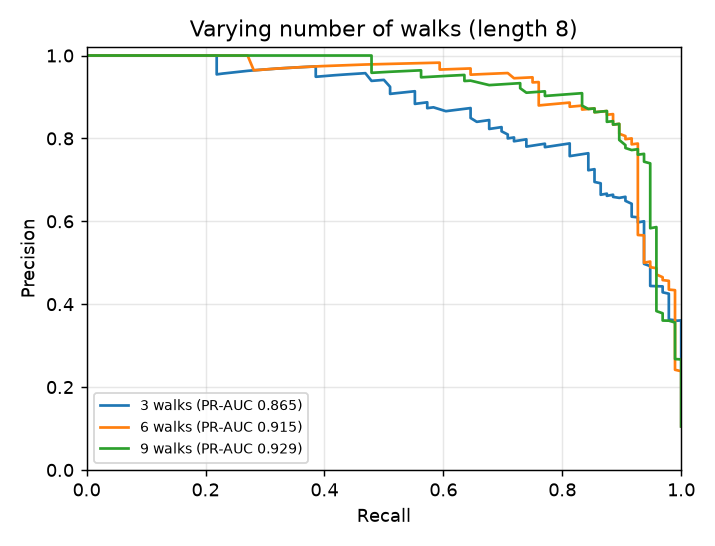
\includegraphics[width=\textwidth]{figures/sweep_fig5_walks}\caption{Number of walks.}\end{subfigure}\hfill
\begin{subfigure}{0.48\textwidth}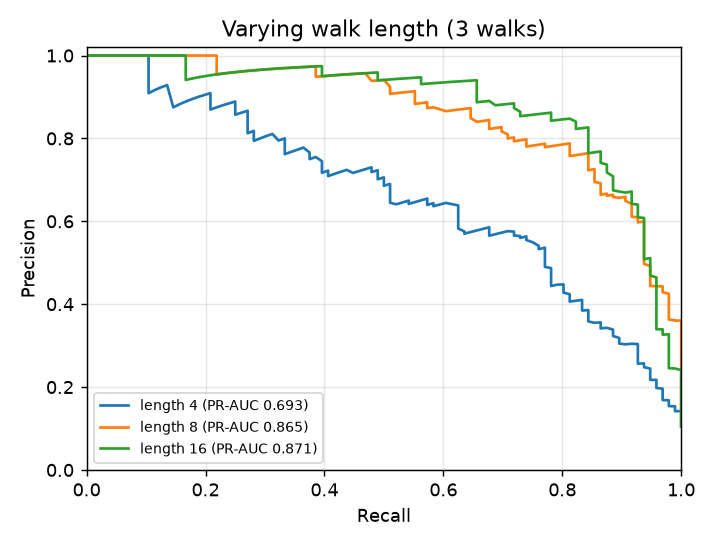
\includegraphics[width=\textwidth]{figures/sweep_fig6_length}\caption{Walk length.}\end{subfigure}\\[4pt]
\begin{subfigure}{0.48\textwidth}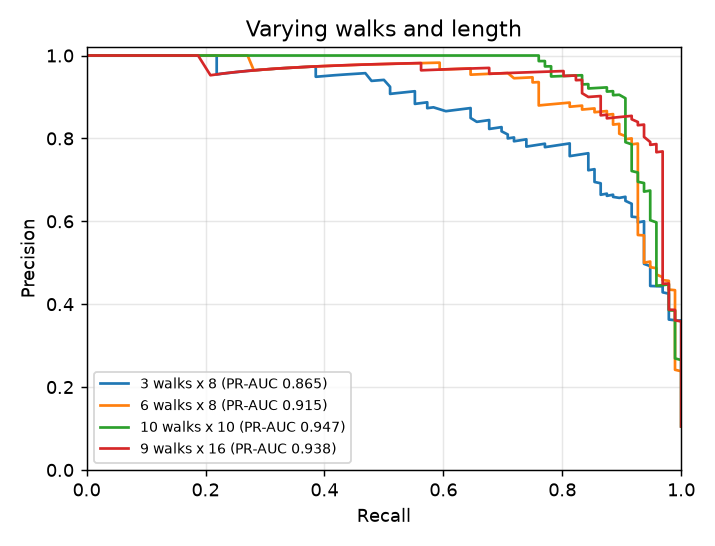
\includegraphics[width=\textwidth]{figures/sweep_fig7_joint}\caption{Walks and length.}\end{subfigure}\hfill
\begin{subfigure}{0.48\textwidth}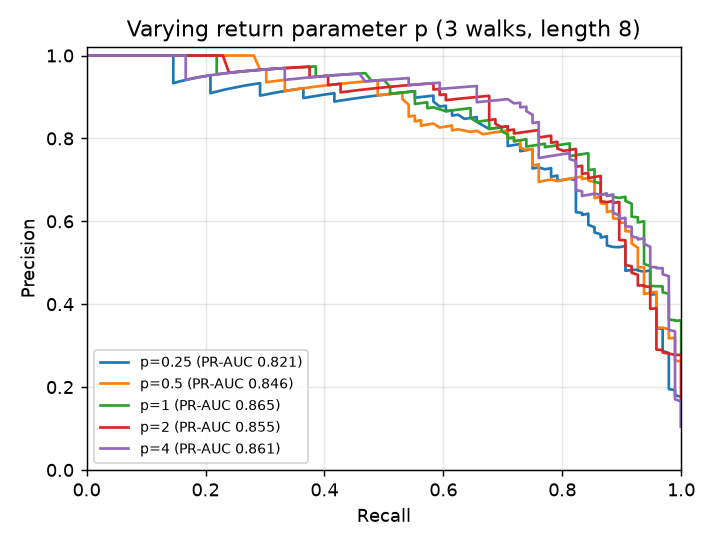
\includegraphics[width=\textwidth]{figures/sweep_fig8_p}\caption{Return parameter $p$.}\end{subfigure}\\[4pt]
\begin{subfigure}{0.48\textwidth}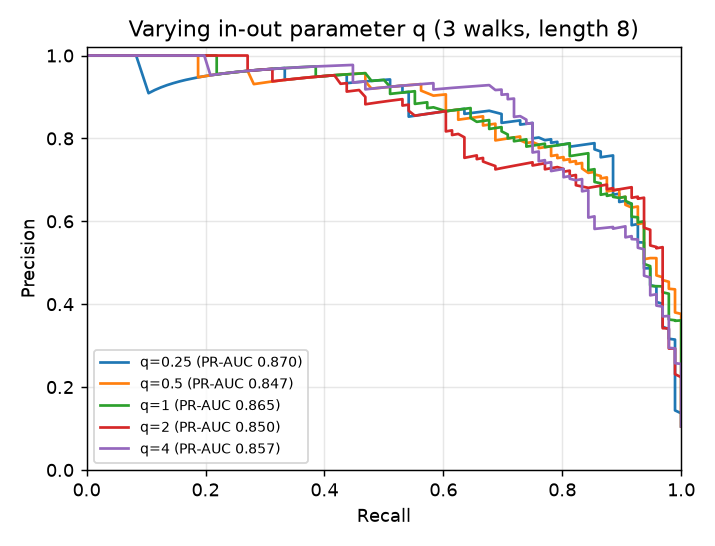
\includegraphics[width=\textwidth]{figures/sweep_fig9_q}\caption{In-out parameter $q$.}\end{subfigure}
\caption{Precision--recall curves of the Table~III sweep (analogs of the paper's Figures~5--9; one curve per setting from the first test split, legends give the mean PR-AUC over five splits).}
\label{fig:sweepcurves}
\end{figure}

\chapter{Full-Page Screenshots}
\label{app:screens}
The following captures show each page of the application at full length.
\shot{02_overview_full}{Overview page, full length.}
\shot{04_system_full}{System page, full length, with the planned modules shown.}
\shot{39_compare_full}{Compare page (phishing case), full length, including the published 20-case table.}
\shotw{41_gaps_full_p1}{Gaps page, first half.}{0.78}
\shotw{41_gaps_full_p2}{Gaps page, second half: remaining gaps and the roadmap.}{0.78}
\shotw{43_report_full_p1}{Investigator report, first half.}{0.78}
\shotw{43_report_full_p2}{Investigator report, second half: evidence paths, laundering patterns, method and limits.}{0.78}

\chapter{Chronological Work Log}
\label{app:log}
This log lists, in order, what was done and observed during the project, including approvals and corrections. It complements Table~\ref{tab:workdone}.
\begin{enumerate}[label=\arabic*.]
\item \textbf{Paper review.} The RiskSEA paper was read; we assessed which parts could be implemented from its text and which depend on private data (labels) or cluster scale.
\item \textbf{Plan.} An end-to-end reproduction workflow was written for execution step by step, with the instruction that every deviation be recorded; a first synthetic world with planted fraud clusters was used to debug before real data.
\item \textbf{Cost control first.} BigQuery dry runs were run before any extraction; the extraction was approved for a specific tier and cost; every query carried a billing cap equal to its dry run plus 5\%.
\item \textbf{Authentication.} Application-default credentials were set up by the user; the code base never handles credentials.
\item \textbf{Label sources.} Public sources were identified; the Etherscan-derived label lists and the OFAC list were downloaded only after explicit approval of each file, and the terms-of-use caveat was recorded (decision D19).
\item \textbf{Extraction and download.} The fast download path was blocked by policy, so parallel resumable REST reads were used; the highest block received was verified to be exactly 5\,000\,000.
\item \textbf{Graph, features, embeddings.} The staged DuckDB graph build replaced a first attempt that ran out of memory; features were log-compressed after a float32 overflow; the gensim integer-token trap was found and fixed.
\item \textbf{Experiments.} Table~II was run in two variants; the has-embedding leak was found and controlled; the Table~III sweep was run on the core subgraph with retraining noise measured; Table~IV was run at three checkpoints; t-SNE figures and cluster metrics were produced.
\item \textbf{Version control.} The user created the repository and made all commits; the assistant supplied commands only.
\item \textbf{Comparative study.} A LaTeX report compared the paper with the reproduction, starting with a comparison of data constraints; its PDF was produced.
\item \textbf{Extension study.} The textbook was read; RiskSEA was judged a strong baseline for scoring and infrastructure but not for tracing and attribution; eight research gaps were written in plain words and the architecture was sketched.
\item \textbf{CryptoTrace build.} Engines, providers, label store, API and interface were built; a dry run of the per-hop query gave 1.2\,GiB; validation on KuCoin and Cryptopia followed (Tornado Cash reached; EtherDelta reached; Yobit.net and OKEx not reached).
\item \textbf{Defects.} The dry-run placeholder, the provider time filter, the parent--child ping-pong, the exploration query over our own cap and several interface bugs were found and fixed (Table~\ref{tab:bugs}).
\item \textbf{Third case.} A real phishing-labeled wallet was found with an exploration query of 29.9\,GiB, traced for 19.9\,GiB, and added as the main demonstration case, with the selection bias disclosed.
\item \textbf{Polish.} Findings were grouped by receiving entity, a demo guide, keyboard shortcuts, automatic highlighting of the top finding, and a responsive layout were added; 78 tests pass.
\item \textbf{Presentation material.} Plain-language explanations of each screen and of the improvements over the baseline were prepared for the project presentation.
\item \textbf{This report.} Screenshots taken earlier were found to mismatch their file names in several cases (wrong strategy or case), so the screenshot script was rewritten and every screen was retaken before they were included.
\end{enumerate}

\end{document}
